\section{Future Prospects}
\label{Sec:Future}
The cornucopia of experimental advances and theoretical insights detailed in Section~\ref{Sec:Progress}
are but a representative sample of the advances made in the field since the last Long Range Plan.
As in all healthy scientific enterprises, our increased understanding of hot QCD matter
has engendered new questions. 
These questions are both quantitative
(``What is the precise value of $\eta/s$ at the various temperatures accessible at RHIC and the LHC?")
and qualitative
(``How does the perfect liquid behavior of quark-gluon plasma emerge from the QCD Lagrangian?")
in nature. 
In addition, opportunities exist to ask and address discovery-oriented
questions, such as ``Does the QCD phase diagram have a critical point?''
The field is poised to answer definitely such questions in the next decade,
thanks to ongoing and anticipated investments in the experimental programs 
at RHIC and the LHC, and in theoretical investigations world-wide. 
This section describes those opportunities and delineates the
progress that will follow from exploiting them.

\subsection{Facilities Evolution}
\label{Sec:FacilitiesFuture}

Planning is well underway to address the compelling physics questions presented in Section~\ref{Sec:Progress}. 
The evolution of the RHIC and LHC accelerators, accompanied by upgrades to their experiments, will provide tools uniquely suited
for determining the inner workings of thermal QCD matter. The prospect of these two facilities, operating with increased luminosity
and a range of energies spanning three orders of magnitude, coupled with greatly upgraded detector capabilities, provides an unprecedented
opportunity to resolve fundamental aspects of QCD.

\begin{figure}[ht]
\centerline{
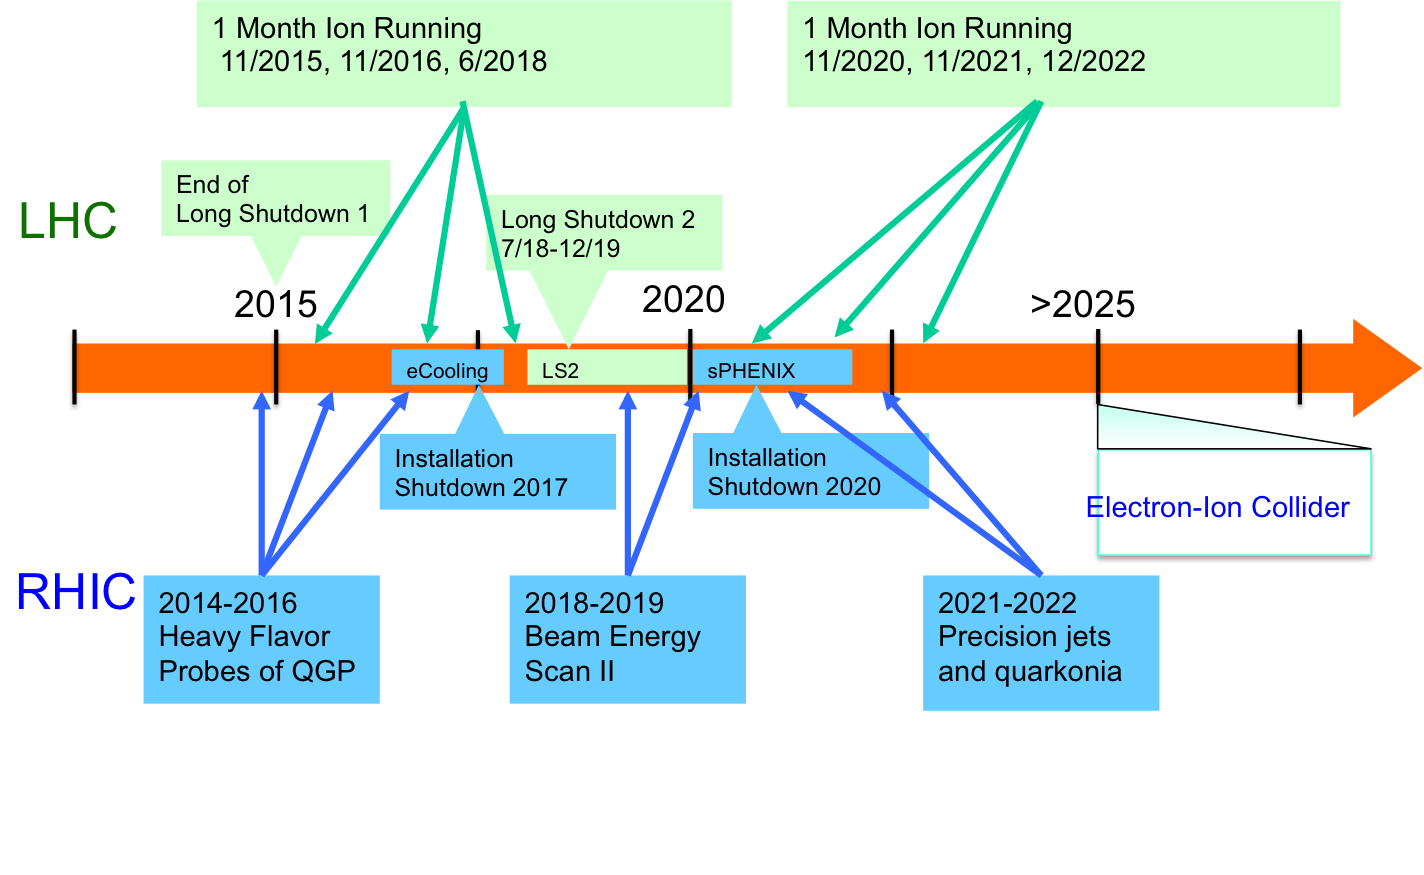
\includegraphics[width=1.00\textwidth]{fig/Timeline.png}
}
\caption{The timeline for future RHIC and LHC heavy ion running.
}
\label{Fig:Timeline}
\end{figure}

\subsubsection{Facility and experiment upgrades at RHIC}
\label{Sec:RHICUpgrades}
At Brookhaven National Laboratory, the goal for the next decade is to complete the  science mission of RHIC on a schedule that permits a smooth and timely transition towards preparations for an electron-ion collider based on the RHIC complex. 
A coherent physics program has been developed to address the outstanding questions in both hot and cold QCD physics 
relevant to completing our understanding of the QGP, with a natural physical and intellectual evolution towards the 
physics addressed by an electron-ion collider.
Accordingly, future heavy ion running is divided into three campaigns: 

\begin{itemize}[leftmargin=2.0cm]

\item[\bf 2014-16:] Measure heavy flavor probes of the QGP using the newly installed silicon vertexing detectors in PHENIX and STAR.
\item[\bf 2018-19:] Conduct a fine-grained scan of the QCD phase diagram via Phase II of the RHIC Beam Energy Scan program.
\item[\bf 2021-22:] Perform precision jet quenching and quarkonia measurements following the installation of sPHENIX.

\end{itemize}

Interspersed between these three running periods are two shutdowns, as illustrated in Figure~\ref{Fig:Timeline}. 
\begin{figure}[!htp]
\centerline{
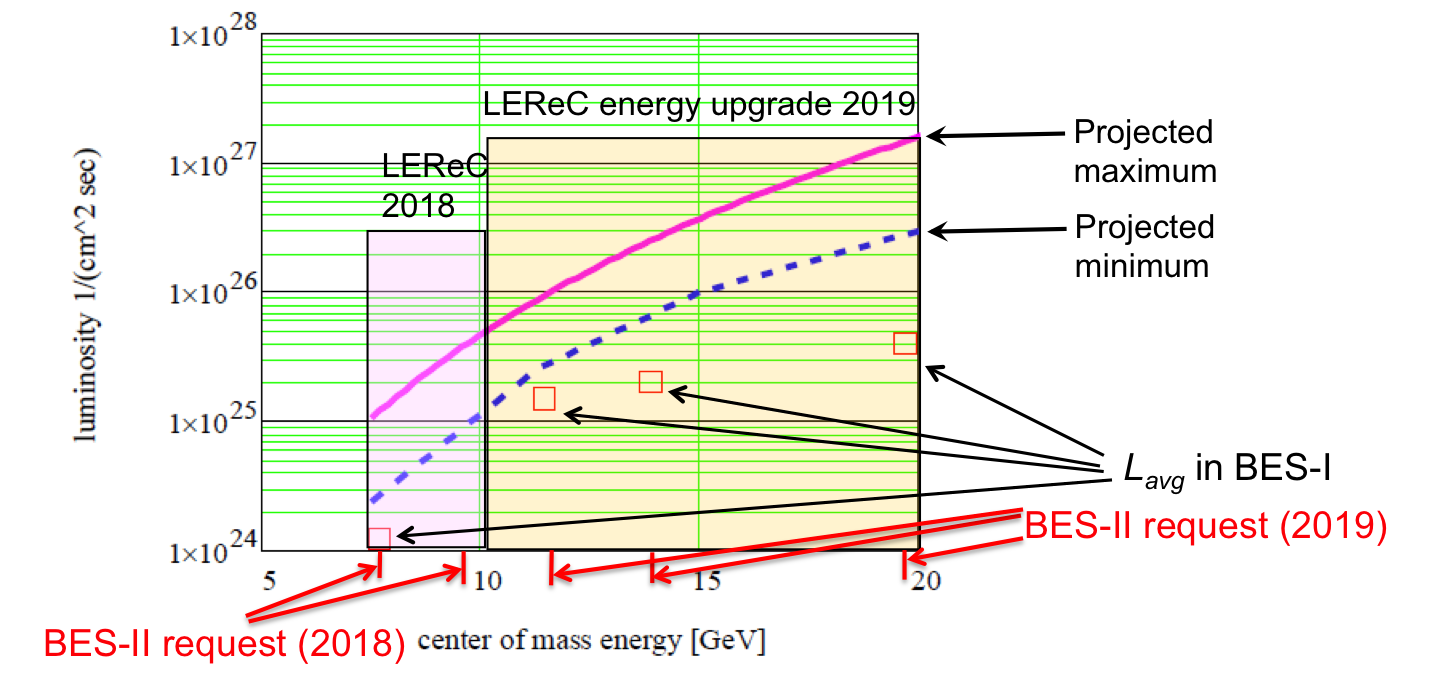
\includegraphics[width=1.00\textwidth]{fig/RHICeCooling.png}
}
\caption[Projected RHIC luminosity increase at low energies from electron cooling]{The projected RHIC luminosity increase at low energies provided by electron cooling of the ion beams. The red squares are the measured average luminosity in RHIC Beam Energy Scan~I. The blue dashed line is the minimum projection for the improvement with electron cooling; the magenta solid line is the maximum projection. Also shown are the actual luminosities achieved in RHIC BES~I. 
}
\label{Fig:eCooling}
\end{figure}
The first shutdown, in 2017,  is to allow for installation of electron cooling to increase RHIC's luminosity
at low energies\footnote{It should be noted that the current RHIC performance at low energies exceeds the original design values for luminosity by well over an order-of-magnitude. In fact, the original RHIC design was limited to energies of 20 GeV and above.}, 
as shown in Figure~\ref{Fig:eCooling}. This luminosity upgrade, in combination with targeted upgrades of the STAR detector described below, greatly increases the discovery potential of the subsequent beam energy scan in 2018-2019. The second shutdown, in 2020, will be used to install the sPHENIX detector (discussed below), prior to a period of dedicated running to explore the microscopic structure of the QGP with high energy jets and quarkonia measurements. Both the sPHENIX upgrade and the proposed STAR upgrades provide natural evolution paths towards detectors for the EIC\footnote{In addition to the upgrade paths from sPHENIX to ePHENIX and STAR to eSTAR, consideration has been given
to a new detector explicitly designed for electron-ion capabilities. Details are available in Refs.~\cite{Accardi:2012qut,Boer:2011fh}
}.

\begin{figure}[!htp]
   \centering
       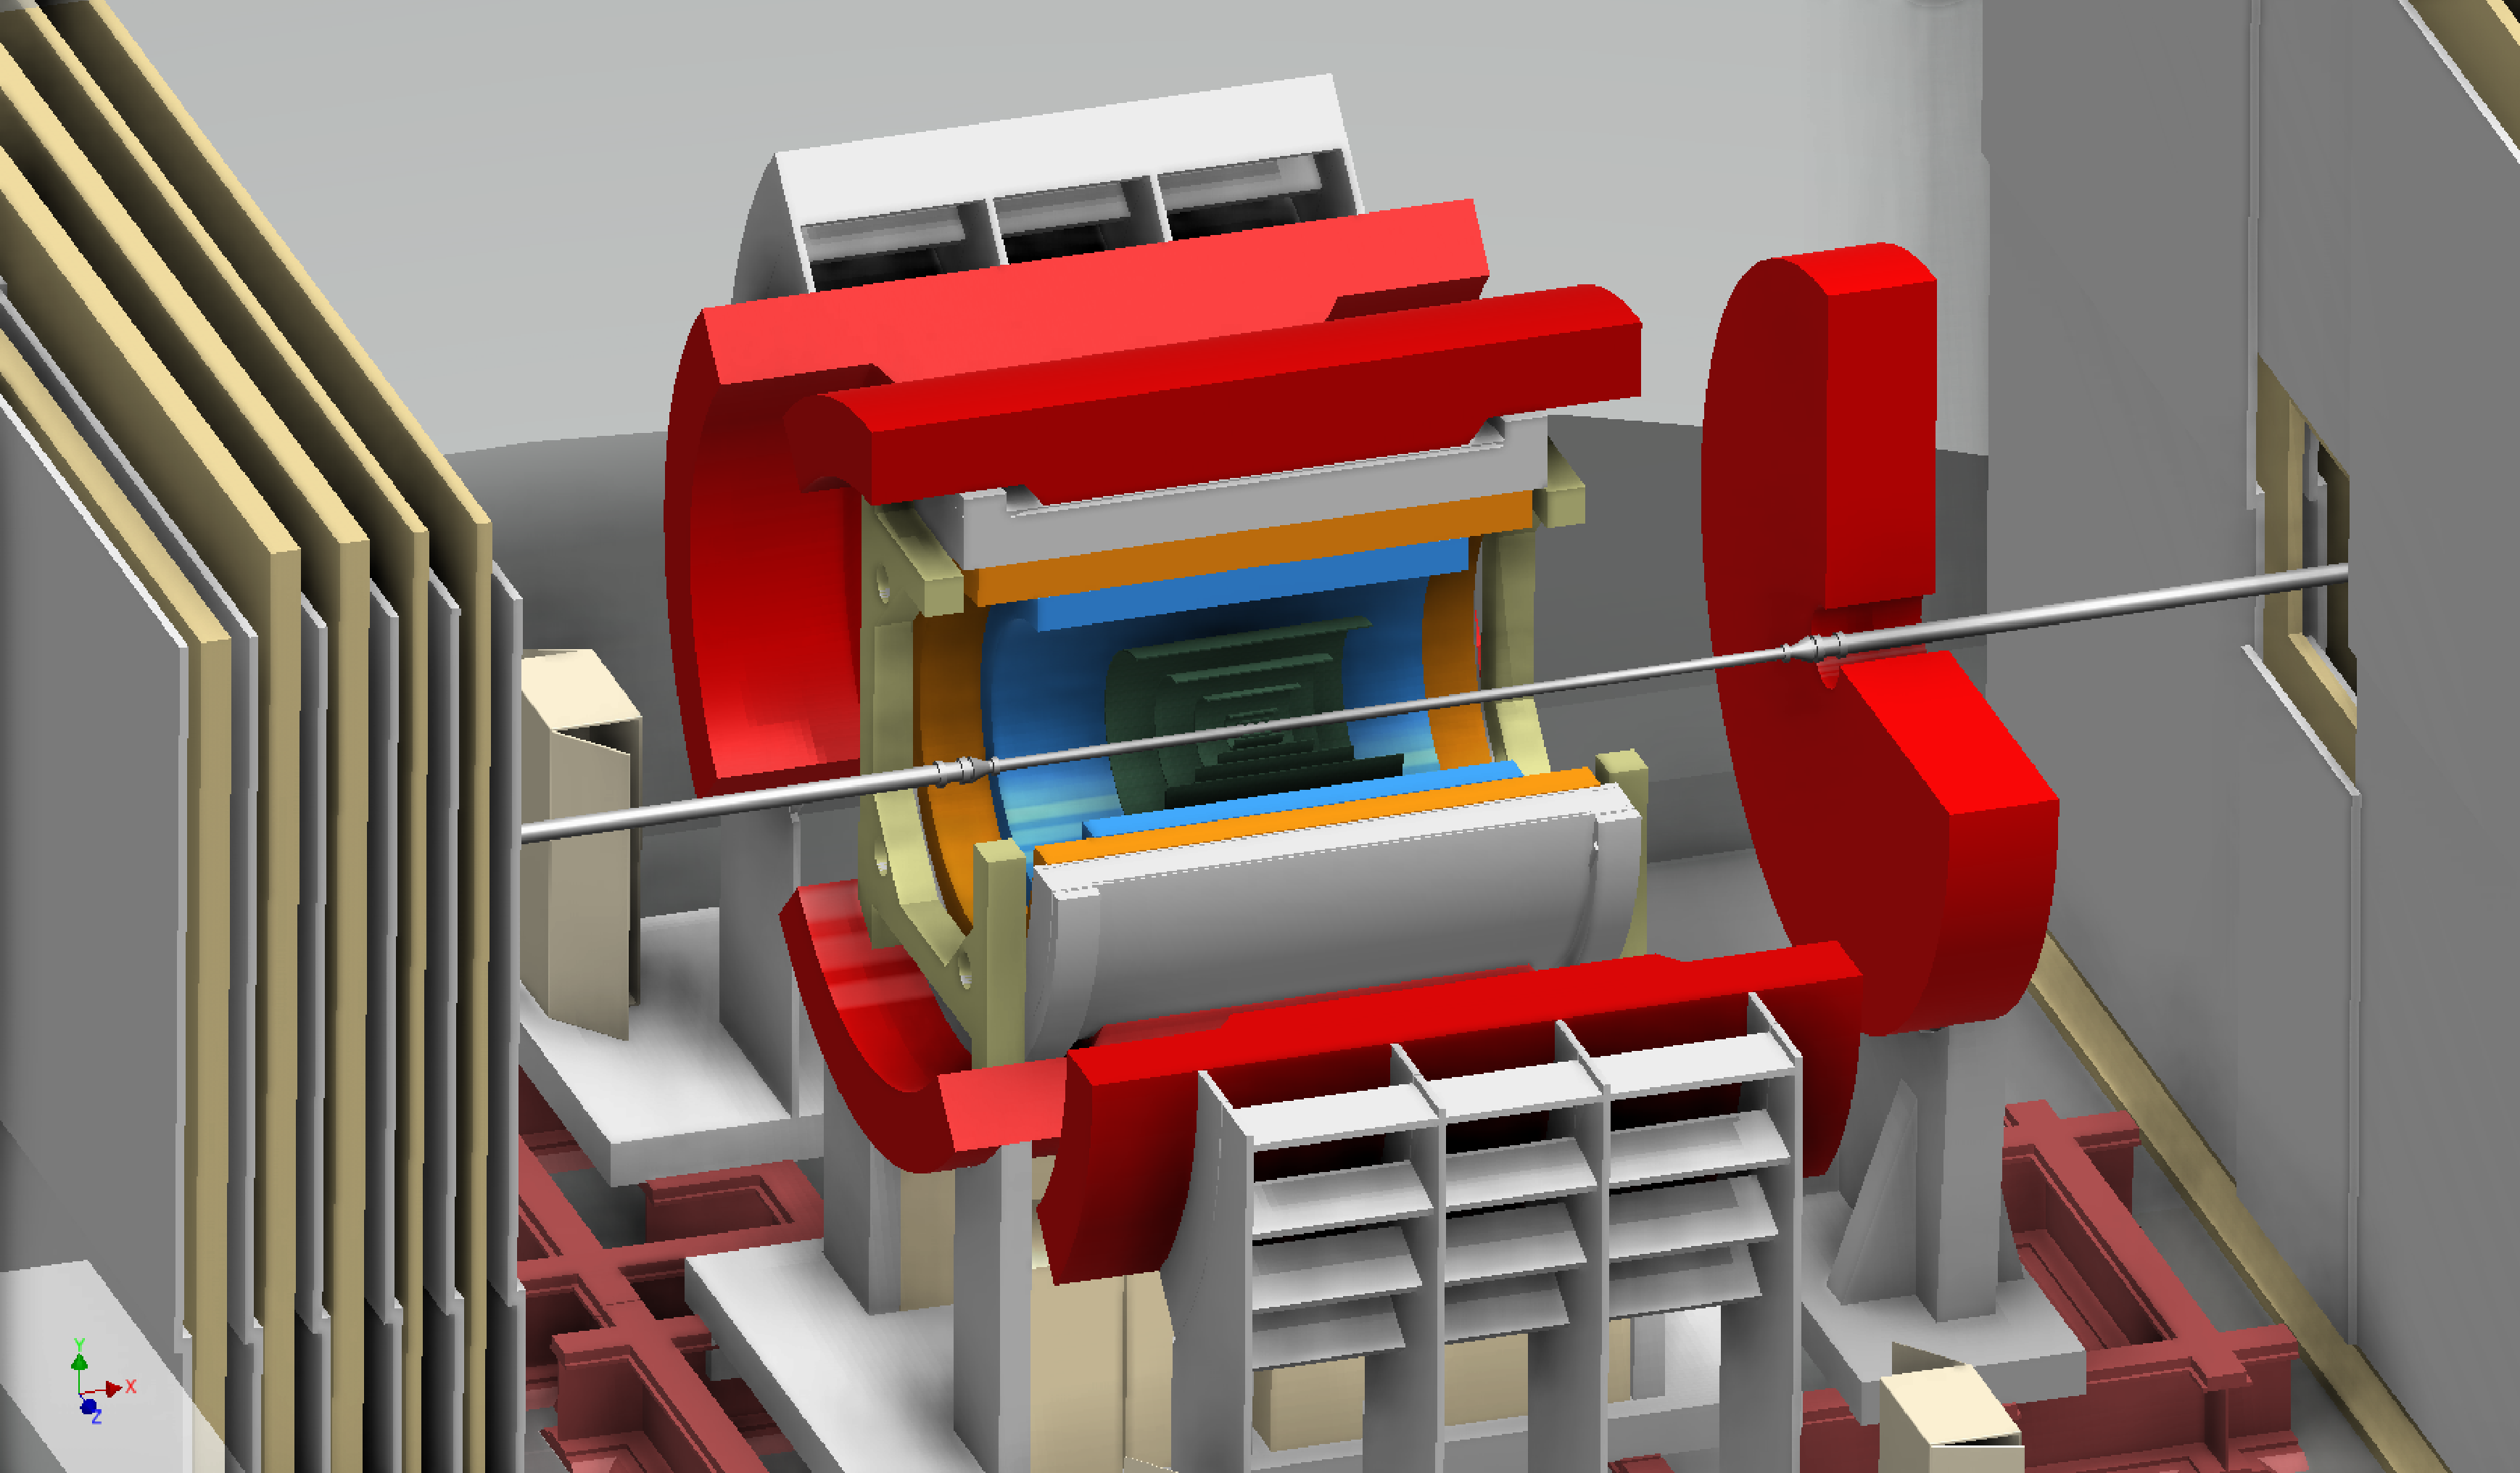
\includegraphics[width=0.9\linewidth]{fig/sPhenix-3D-Hall-Cutout.pdf}
       \vskip 4mm
       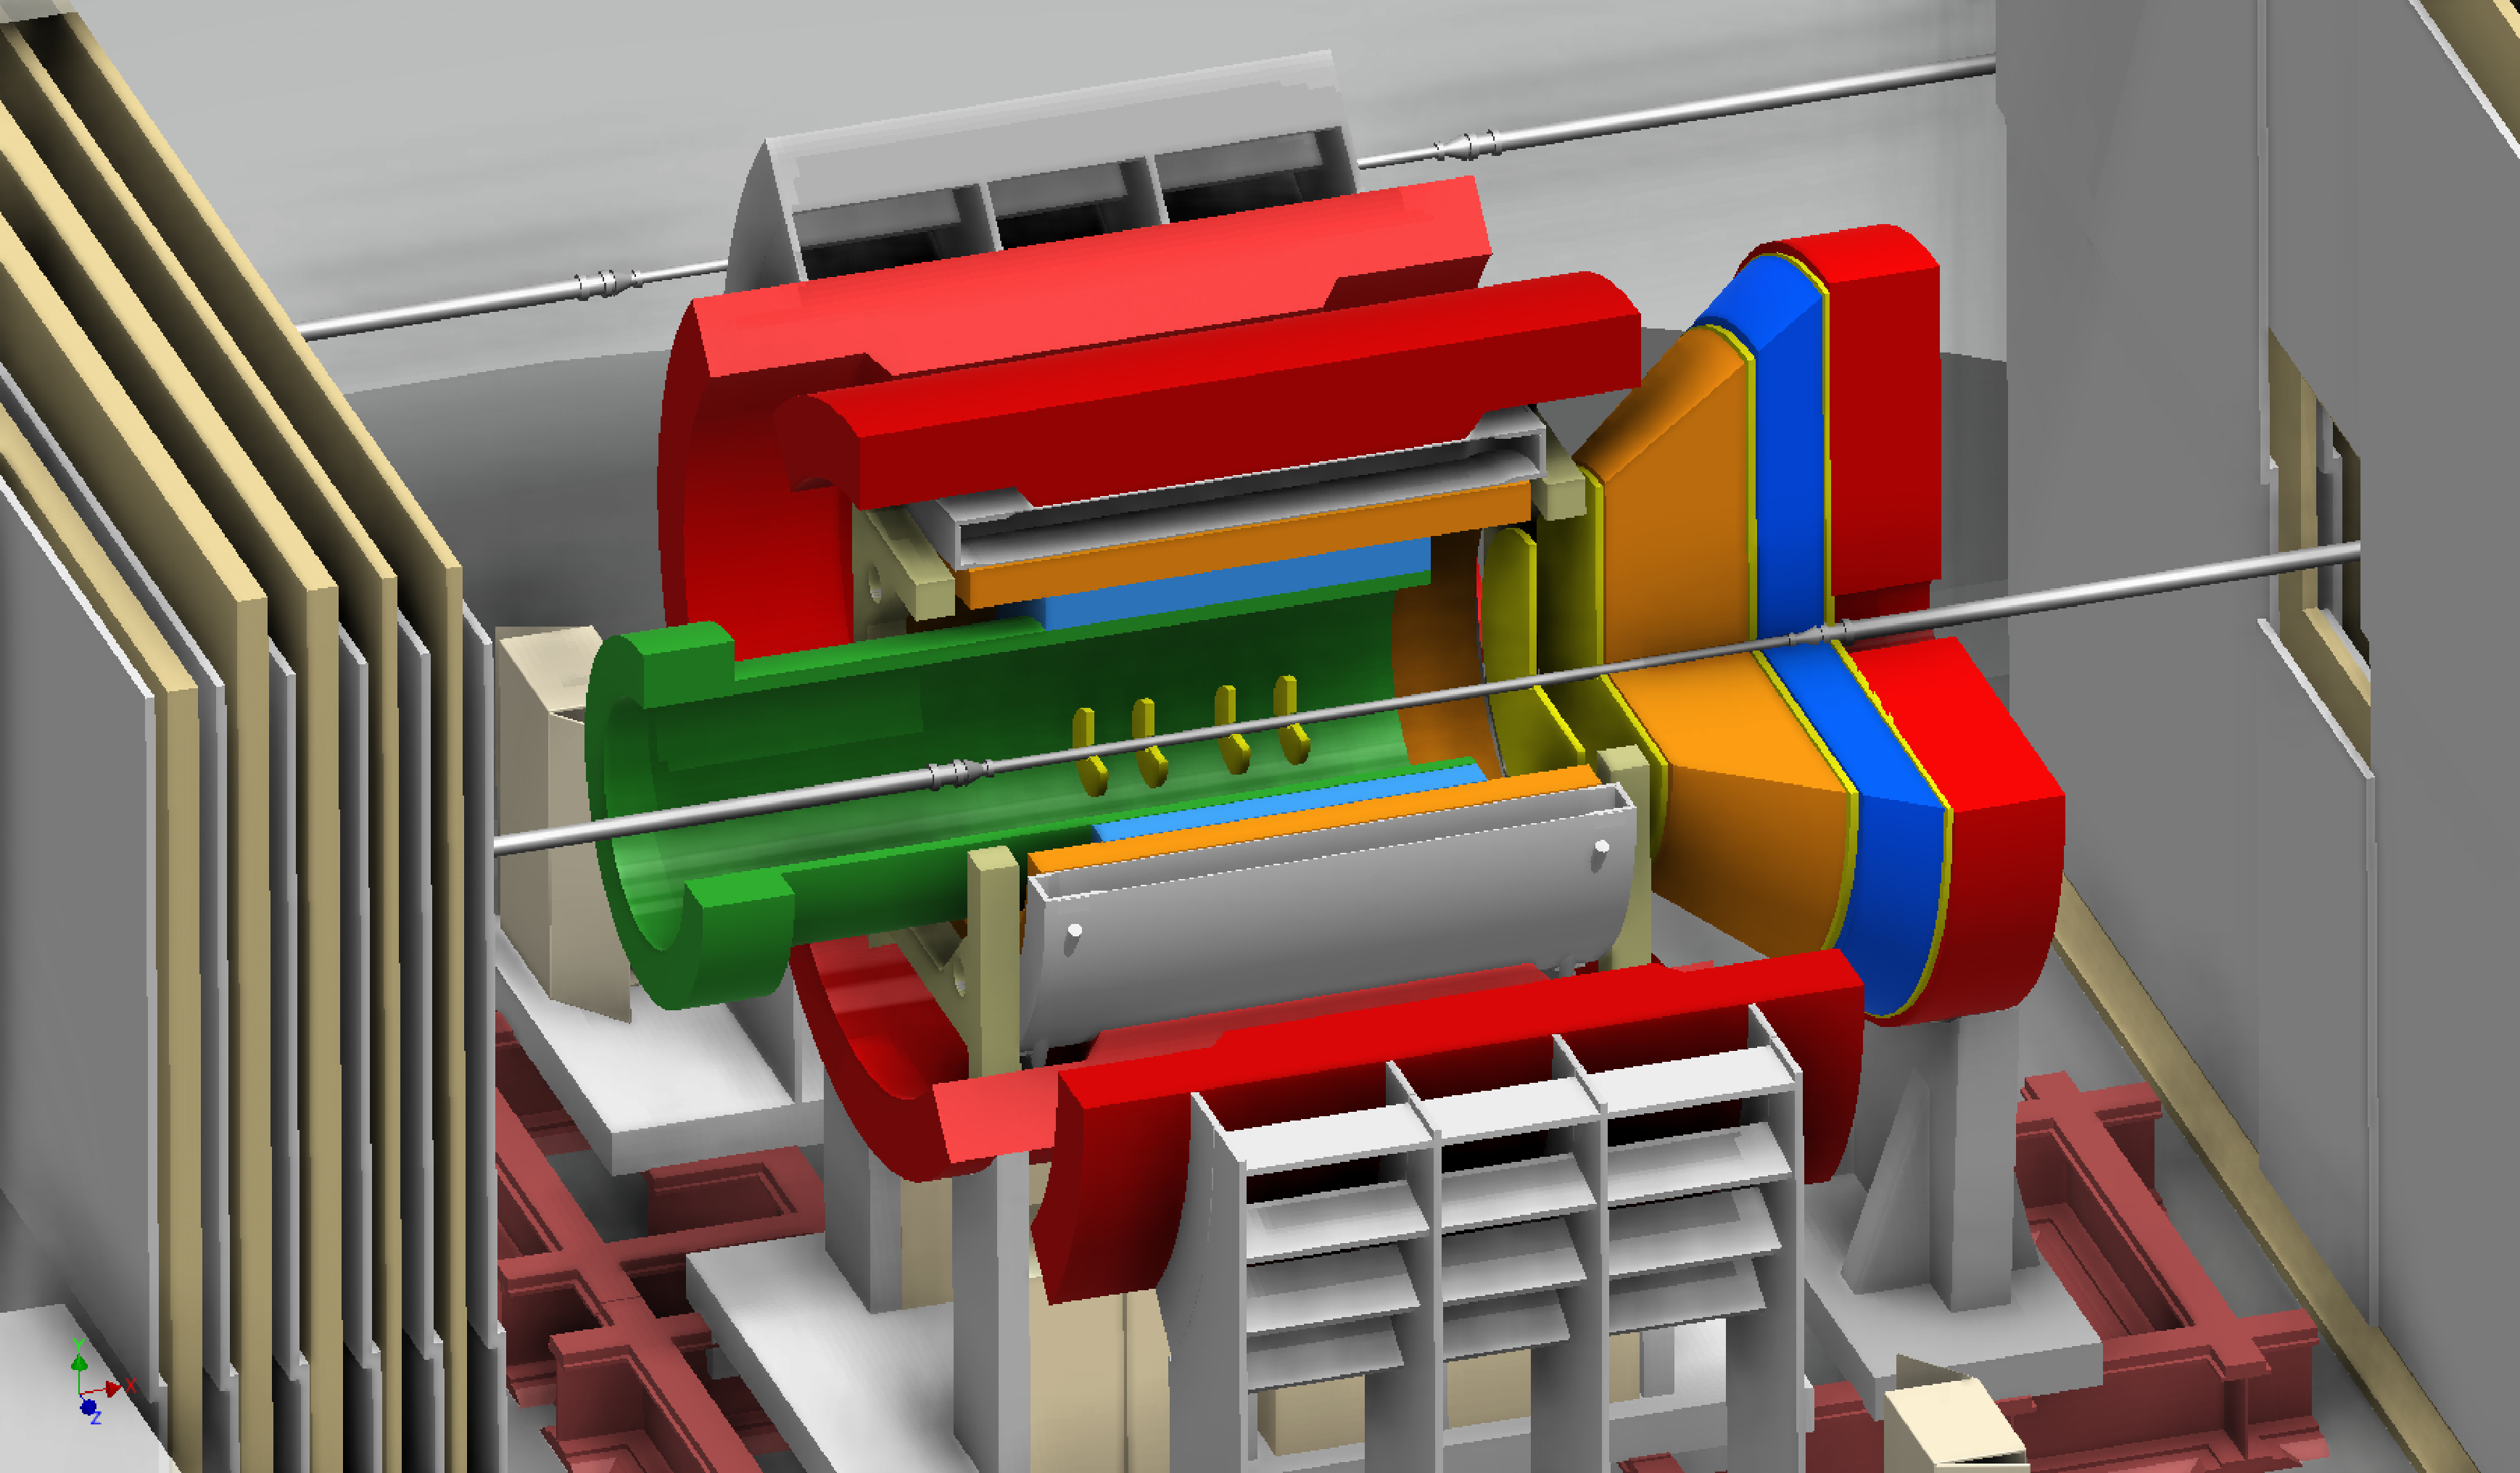
\includegraphics[width=0.9\textwidth]{fig/ePhenix-Cut-Out-View.pdf}
       \caption[Proposed sPHENIX upgrade and its evolution to an EIC detector]{ (top) An engineering rendering of the proposed
         sPHENIX upgrade to the PHENIX experiment, showing the inner
         tracking system, the electromagnetic calorimeter, the BaBar
         solenoid and the hadronic calorimeter. (bottom) The evolution
         of the sPHENIX detector into a full-capability EIC detector.}
       \label{Fig:sPHENIX}
       \label{Fig:ePHENIX}
\end{figure}

{\bf sPHENIX:} The PHENIX collaboration has submitted a
proposal\cite{Aidala:2012nz} to the DOE for MIE funding (Major Item of
Equipment) to replace the PHENIX central detectors in order to provide
full hadronic and electromagnetic calorimetry along with charged
particle tracking over a pseudorapidity interval $\eta < 1$ The new
apparatus, sPHENIX, shown in Figure~\ref{Fig:sPHENIX} would
dramatically extend the range of jets measurable at RHIC and provide
precision spectroscopy of quarkonia.  With a mass resolution of better
than 100~MeV/$c^2$, sPHENIX will separately measure the $1S$, $2S$ and
$3S$ states of the upsilon, providing key information about Debye
screening in the QGP.  The full sPHENIX physics program employs
inclusive jet, dijet, $b$-tagged jet, $\gamma$$+$jet, high transverse
momentum charged hadron, jet fragmentation function, and upsilon
measurements to enable a very comprehensive and detailed investigation
of the microscopic dynamics of the QGP in the temperature range where
its coupling is at its strongest.

The very high data acquisition bandwidth of sPHENIX, combined with
RHIC~II luminosities, brings fundamentally new capabilities to the
measurement of hard probes at RHIC.  In one year, sPHENIX will record
100 billion minimum bias Au$+$Au collisions, providing an extremely
large sample of unbiased jets.  This enormous sample will be further
augmented by calorimetric triggers sampling more than 2/3 of a
trillion top-energy Au$+$Au collisions made possible by the RHIC~II
luminosity.  All told, this enables the measurements of jets in
$p$$+$$p$, $p$$+$Au and Au$+$Au beyond 70~GeV and a correspondingly
large kinematic reach for other hard probes, as shown in
Figure~\ref{fig:AAphysics_projections}.

\begin{figure}[hbt!]
  \centering
  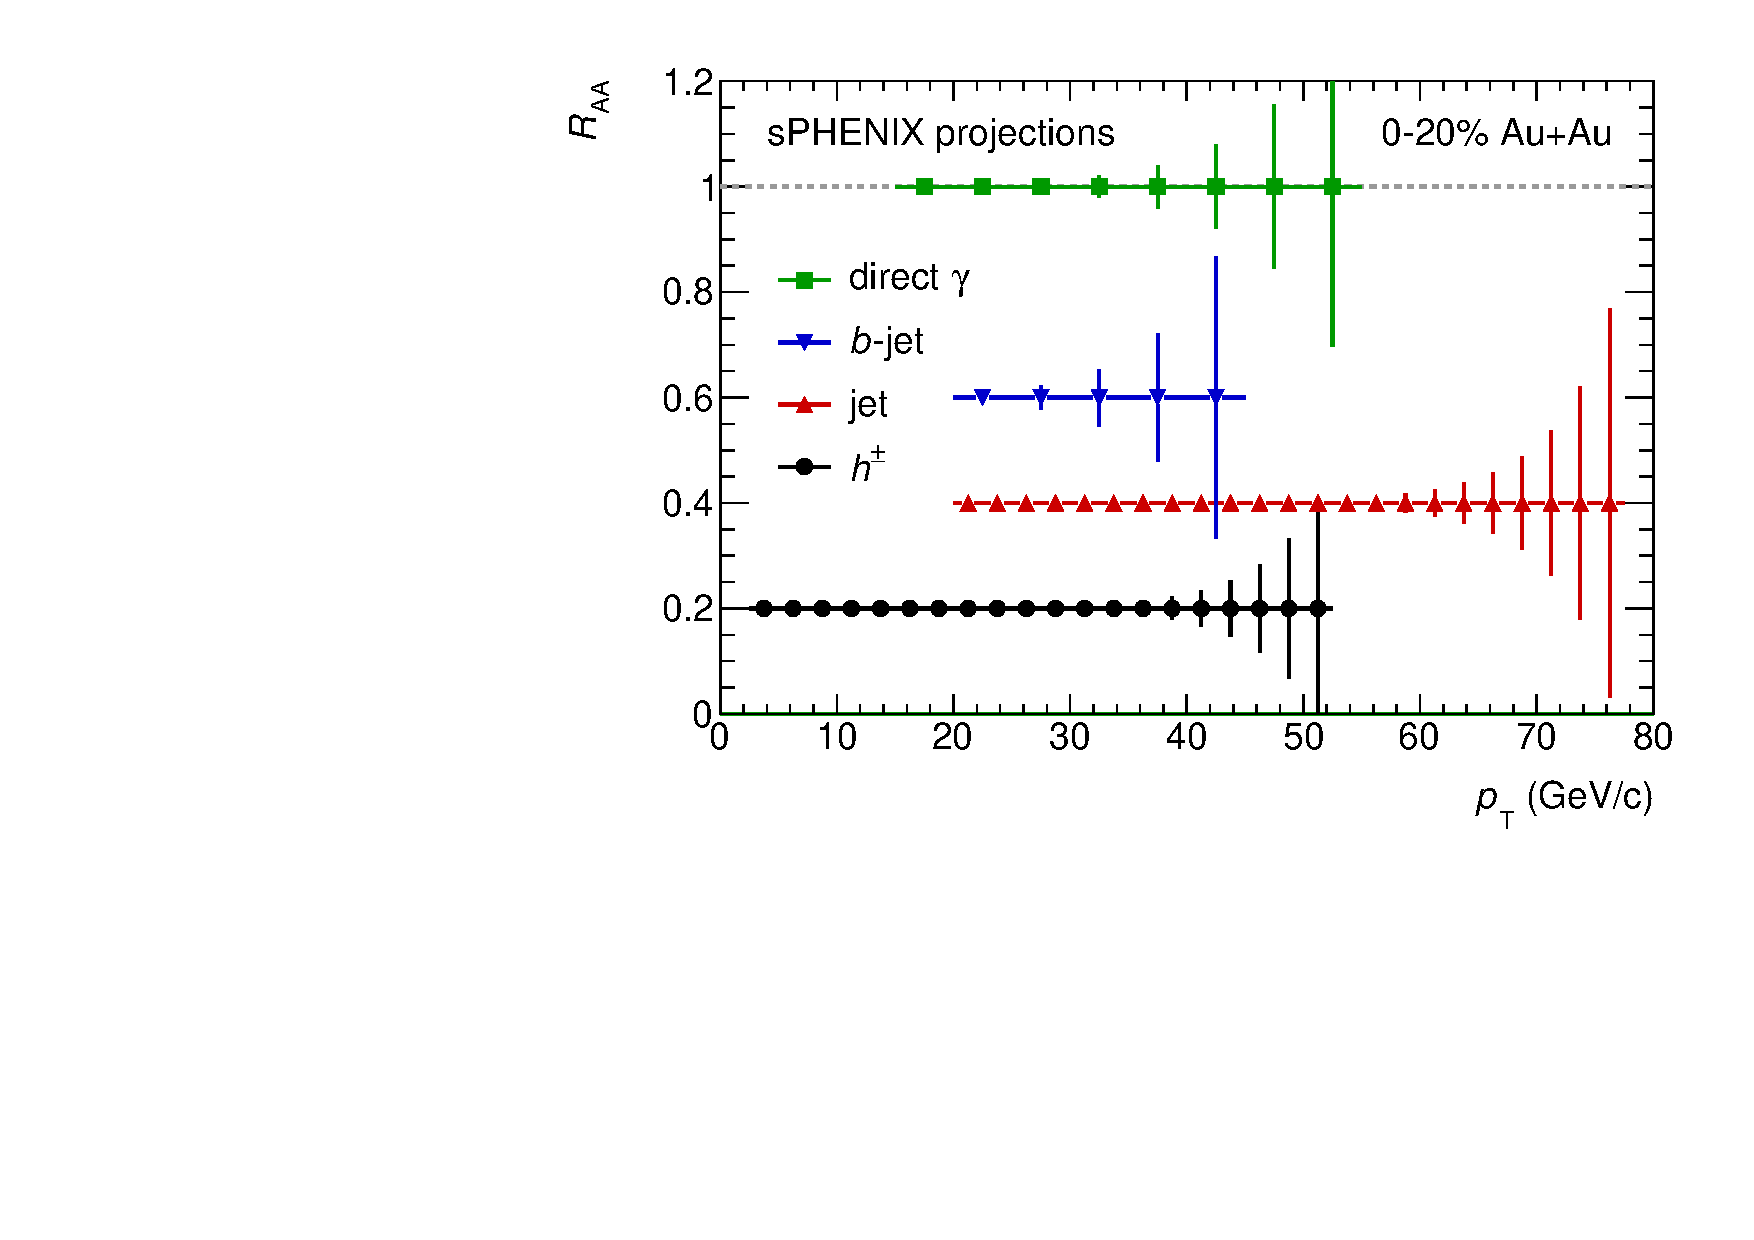
\includegraphics[width=0.8\textwidth]{fig/sPHENIX_MIE_master_AuAu_projections}
  \caption[Projected sPHENIX statistical uncertainties on $R_\mathrm{AA}$
    for $\gamma$'s, jets, $b$-jets and $h^\pm$]{Projected statistical uncertainties on the $R_\mathrm{AA}$
    for inclusive photons (green points, assuming $R_\mathrm{AA} =
    1$), $b$-jets (blue points, assuming $R_\mathrm{AA} = 0.6$),
    inclusive jets (red points, assuming $R_\mathrm{AA} = 0.4$) and
    charged hadrons (black points, assuming $R_\mathrm{AA} =
    0.2$). These projections are made with a $b$-jet tagging
   efficiency of $50$\%, 10 weeks of $p$+$p$ and 22 weeks of Au$+$Au
    data taking.}
    \label{fig:AAphysics_projections}
\end{figure}

This reach in $Q^2$, combined
with precision vertexing provides the basis for a compelling program of direct comparisons to corresponding measurements at the LHC
discussed in Sections~\ref{Sec:FutureJetCapabilities}, \ref{Sec:FutureJetProbes} and \ref{Sec:FutureQuarkonia}. The sPHENIX design takes advantage of recent technological advances in sensors and read-out electronics to minimize costs. In addition, the superconducting solenoid from the BaBar experiment at SLAC has been transferred to BNL\cite{BabarMove} for use in sPHENIX, resulting in a very considerable cost savings. Finally, the sPHENIX design provides a route for a smooth evolution to a full-capability EIC detector\cite{Adare:2014aaa}, shown in Figure~\ref{Fig:ePHENIX}. In addition, there is a an exciting extended program of polarized p+p and p+A\cite{PHENIXpppA,Aschenauer:2015eha}
if some of the EIC detector can be realized earlier.

{\bf STAR Upgrades:} The STAR experiment has recently installed two new detector sub-systems: the Heavy Flavor Tracker discussed in Sections~\ref{Sec:Facilities} and Section~\ref{Sec:OpenHF}, and the Muon Telescope Detector described in Section~\ref{Sec:Quarkonia}.
With the completion of the HFT and the MTD,
STAR's upgrade plans next focus on  Phase II of the RHIC Bean Energy Scan.  The inner sectors of the TPC will be replaced to allow full coverage of pads increasing the pseudorapidity coverage, and extending momentum coverage to lower \pT\ . In addition STAR will  add an event plane detector which will enrich the STAR BES program by allowing for an independent measurement of the event plane  and significantly improving its resolution .  Both these and longer term upgrades improve STAR's forward capabilities 
in preparation for an eSTAR configuration in the EIC era\cite{STAR:eSTAR} as outlined in Figure~\ref{Fig:STARplan}.  
\begin{figure}[!htp]
\includegraphics*[width=0.9\textwidth]{fig/starplan_jan2015.pdf}
\vspace{-0.5cm}
\caption[STAR upgrade plan towards an EIC detector]{The STAR upgrade plan,
showing the evolution from the current configuration focused on \pp\ and \AplusA\ physics at
mid-rapidity to a design emphasizing forward physics in \pp\ and \pA\ collisions\cite{STAR:FU,STAR:DecadalPlan}
and later  $e$+p and $e$+A physics at an EIC~\cite{STAR:eSTAR}.}
\label{Fig:STARplan}
\end{figure}

The STAR near-term proposed upgrades relevant to BES-II include:
\begin{itemize}
\item[] {\bf iTPC upgrade:} The STAR collaboration has proposed to upgrade the inner sectors of the read-out plane of the Time-Projection-Chamber (iTPC)~\cite{STAR:BESII}  in order to increase the segmentation on the inner pad plane and to renew the inner-sector wires. This upgrade will improve the resolution on both momentum and $dE/dx$ resolution, increase the track reconstruction efficiency and extend the  acceptance in 
pseudorapidity  from $|\eta| \le 1.1$ to $|\eta| \le 1.7$.
%Although iTPC will allow significantly improved tracking and coverage out to $|\eta| \le$ 1.7, the longitudinal boost for higher rapidity particles shifts the low $p_T$ particles into a momentum range where it becomes increasingly challenging to employ PID through relative ionization in the TPC. 
The enhanced performance made possible by the iTPC will not only benefit the BES-II physics program but will also be crucial for STAR�s future program with \pp\ / \pA\ and $e$+p/$e$+A collisions at the forward high-rapidity regions.

\item[] {\bf EPD:} The proposed Event Plane Detector (EPD) is a dedicated event-plane and centrality detector placed in the forward rapidity region 2 $\le | \eta| \le$ 4. With segmentation in both radial and azimuthal directions, the detector will provide precise measurements of the collision centrality and the event plane, as well as serving as a trigger detector for collisions at lower beam energies.
%The proposed EPD configurations with 12 or 30 ?-segmentations are both very close to the optimal case. 
The EPD will be crucial for the physics measurements of collectivity as well as correlations in a much wider rapidity region. 
\end{itemize}

In the longer term STAR has proposed a series of mid-rapidity and forward upgrades that are complementary to the sPHENIX
physics program described above. The planned upgrades include:
\begin{itemize}
\item {\bf HFT$^+$:} The current HFT pixel integration time of $\sim 200~\mu$sec is much longer 
than the $\le 40~\mu$sec of the STAR TPC . 
In order to synchronize the TPC and HFT read-out for maximum rate capability for measuring bottom quark production at RHIC, the STAR collaboration has started design studies on the HFT$^+$, a faster version of the HFT with the state of art pixel technology. 
New technological developments permit read-out times less than
$20~\mu$sec without any increase of power consumption, so that the HFT support infrastructure
for cooling and power can be re-used for the HFT$^+$, making it a very cost-effective upgrade. 
%The HFT$^+$ allows tagging of bottom hadron productions at the top RHIC energies. 
The physics enabled by the HFT$^+$ physics is complementary to sPHENIX's jet program as well as ALICE's upgraded heavy flavor program
(to begin in 2019) at the LHC. In addition, the faster HFT$^+$ will be helpful for the heavy flavor physics in the spin program at RHIC.

{\bf Forward Upgrades:} The STAR collaboration has developed plans~\cite{STAR:FU,STAR:DecadalPlan} for measurements with forward photons, $J/\Psi$'s, Drell-Yan pairs, and di-jet and hadron/jet correlation probes, as well as $W$ and $Z$ bosons at top RHIC energy.
%and demonstrate measurement capability and sensitivity through detailed simulations. It will be shown that these probes allow addressing fundamental aspects of the nucleon partonic structure, which are still rather poorly determined by experiment. One is the nature of the nucleon spin; the other is go beyond our current simple one-dimensional picture of nucleons by correlating the information on the individual parton contribution to the spin of the nucleon with its transverse momentum and spatial distribution inside the nucleon. 
Measuring these probes in \pA\ collisions will further our understanding of cold nuclear matter effects in QCD processes in cold nuclear matter by studying the dynamics of partons at very small and very large momentum fractions $x$ in nuclei, and at high gluon density to investigate the existence of nonlinear evolution effects. STAR's forward upgrade plan is centered around the unique capabilities afforded with the existing STAR detector, complemented with detector upgrades including the forward calorimetric system (FCS) and forward tracking system (FTS), which are required to carry out the proposed physics program at forward rapidities. The proposed FCS and FTS upgrades were first envisioned in the STAR Decadal Plan~\cite{STAR:DecadalPlan} and represent a natural evolution of the growth of the STAR scientific program. These upgrades will be an integral part of the eSTAR configuration at eRHIC outlined in the eSTAR letter of intent~\cite{STAR:eSTAR}, see Figure~\ref{Fig:eSTAR}.
\begin{figure}[!htp]
\includegraphics*[width=0.9\textwidth]{fig/estar_proposal.pdf}
\vspace{-1.5cm}
\caption[eSTAR layout with proposed upgrades]{eSTAR layout with the proposed upgrades of the iTPC, Forward Calorimetry System (FCS), Forward Tracking System (FTS), Endcap TOF (E/W TOF), BSO Crystal Calorimeter (CEMC), and a GEM-based transition radiation detector. In this configuration, the electron beam is from right to left while hadron beam from left to right~\cite{STAR:eSTAR}. }
\label{Fig:eSTAR}
\end{figure}
\end{itemize}



\subsubsection{Facility and experiment upgrades at the LHC}

Following the successful Run I p+p, Pb+Pb and p+Pb data taking periods, the LHC is now preparing
for Run II, forseen to include p+p, p+Pb and heavy ion data taking from 2015 to 2018. Run II
will be followed by a shutdown from 2018 to 2020 (LS2) and Run III from 2020 to 2023.
For both the p+p and Pb+Pb data taking, the LHC upgrades during the current shutdown should
allow for collisions at close to the design energy, i.e., $\sim$5~TeV for Pb+Pb. In addition, a
large increase in the Pb+Pb instantaneous luminosity is projected, with collision rates expected
to exceed those achieved in Run I by up to one order of magnitude. Combining Run II and III,
the LHC goal is to deliver about 10~nb$^{-1}$  of Pb+Pb collisions to each of ALICE, ATLAS and CMS. In combination,
the increased collision energy and luminosity will increase statistics for rare high \pT\
probes by about a factor of 200.

To exploit the improved accelerator performance, ALICE, ATLAS and CMS are undergoing
significant upgrades during the current shutdown and in the future LS2. For ATLAS and CMS, these upgrades
are mostly driven by the needs of the p+p program. Further large luminosity increases for
\pp\ will produce a larger number of collisions per bunch crossing (``pileup''), eventually
reaching multiplicities per event that are within a factor of 2 of average heavy-ion
collisions. This will require extension (e.g., adding a fourth pixel tracker layer)
and eventually replacement of the silicon inner tracker detectors of the two experiments to
cope with the increased particle densities. In addition, the rejection power of the
trigger systems is being improved by increasing the trigger granularity at the
hardware (L1) level. Both the inner tracker and trigger upgrades, as well as other
developments, are well matched to the needs of the heavy ion program in Run II and III. Of
particular importance is the improved trigger selectivity for jets in central events at L1,
which is essential to fully sample the expected collision data for jet-related probes.

ALICE is preparing for Run II with an expansion of the calorimetric coverage (EMCAL) which will allow for dijet studies and improved jet triggering. During LS2 the experiment's data taking capabilities will be significantly enhanced with major upgrades to detector readout and data acquisition systems  to allow the collection of data at the full collision rate. This includes in particular a replacement of the TPC readout with faster detectors and electronics. In
addition, a replacement of the silicon inner tracking system which would improve precision, acceptance and readout speed has been proposed as well as a proposal to add a silicon telescope in front of the current forward muon detector to improve the low \pT\ momentum resolution of the reconstructed muons. While the main physics driver for the upgrades is precision measurements of the low \pT\ open heavy flavor
program studying e.g.\ charm production and equilibration, these upgrades also benefit the
intermediate and high \pT\ jet quenching program.



\subsection{Mapping the Crossover and Searching for the QCD Critical Point}
\label{Sec:CP}


%
%%%%%%%%%%%%%%%%%%% Figure PD2 %%%%%%%%%%%%%%%%%%%%%%%%%%%%%%%%%%%%
%\begin{figure}[h!]
%\begin{center}
%\begin{minipage}{0.5\textwidth}
%\hspace*{-12mm}
%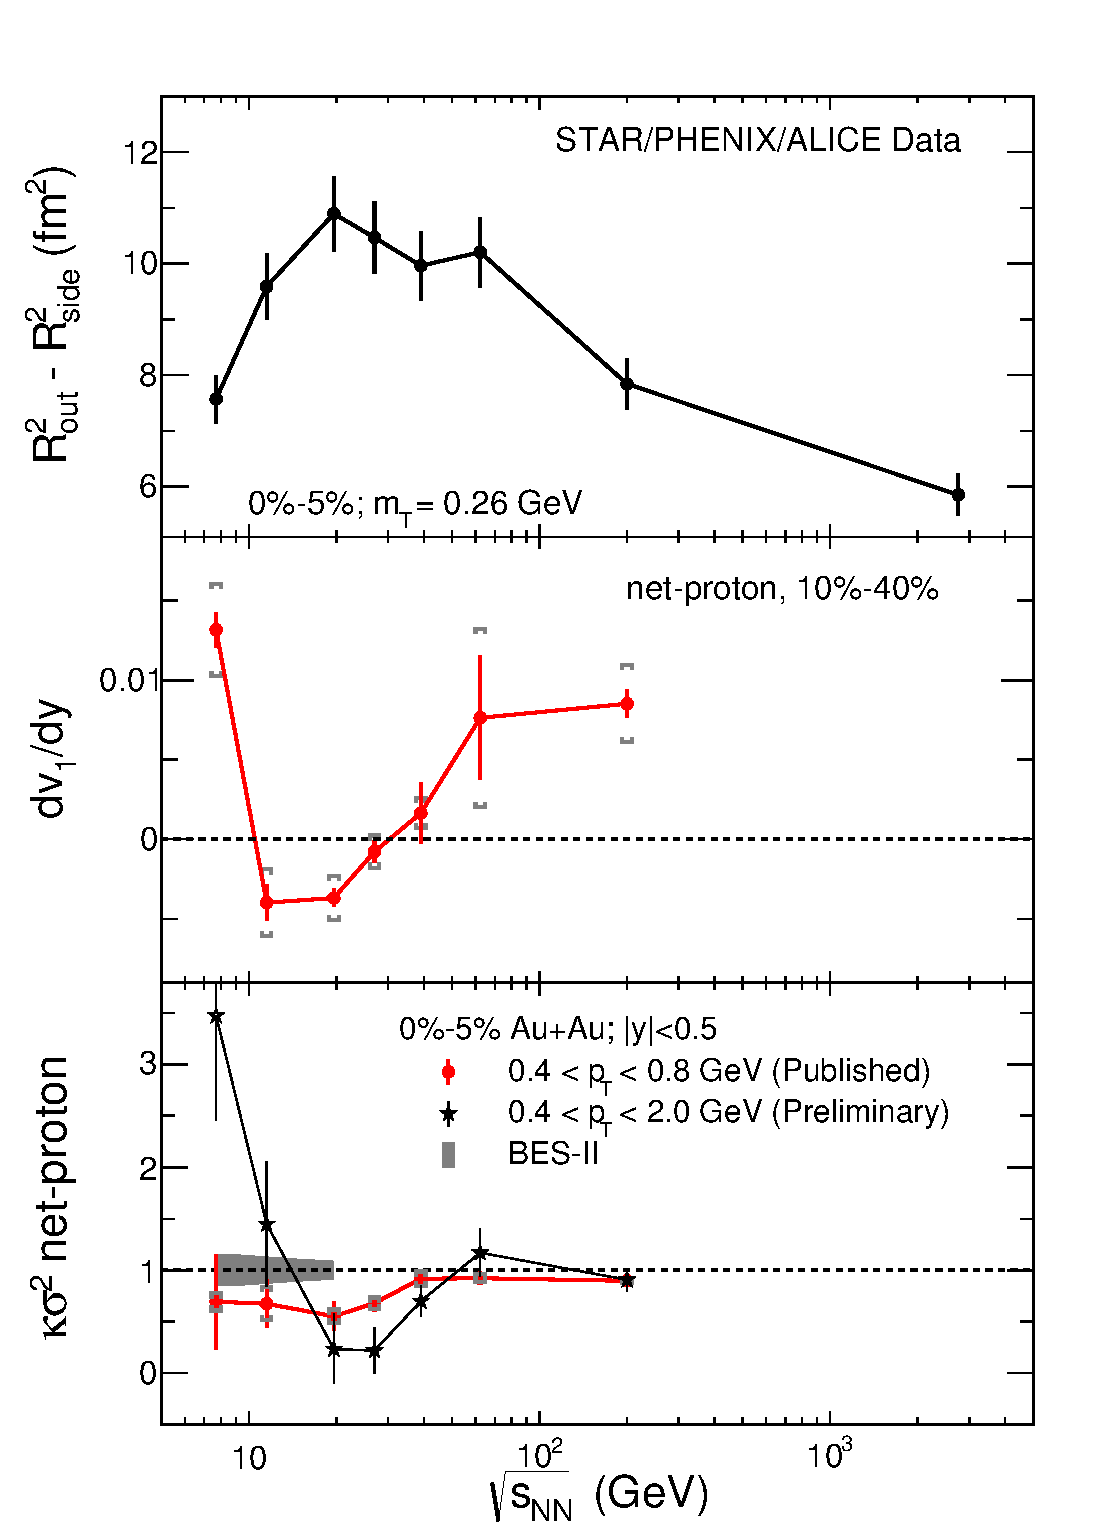
\includegraphics[width=1.22\textwidth]{./fig/bes_compilation_prl_cpod.png}
%\end{minipage}
%\hspace*{2mm}
%\begin{minipage}{0.47\textwidth}
\begin{figure}[!thp]
\vspace{-0.3in}
\begin{center}
\centerline{  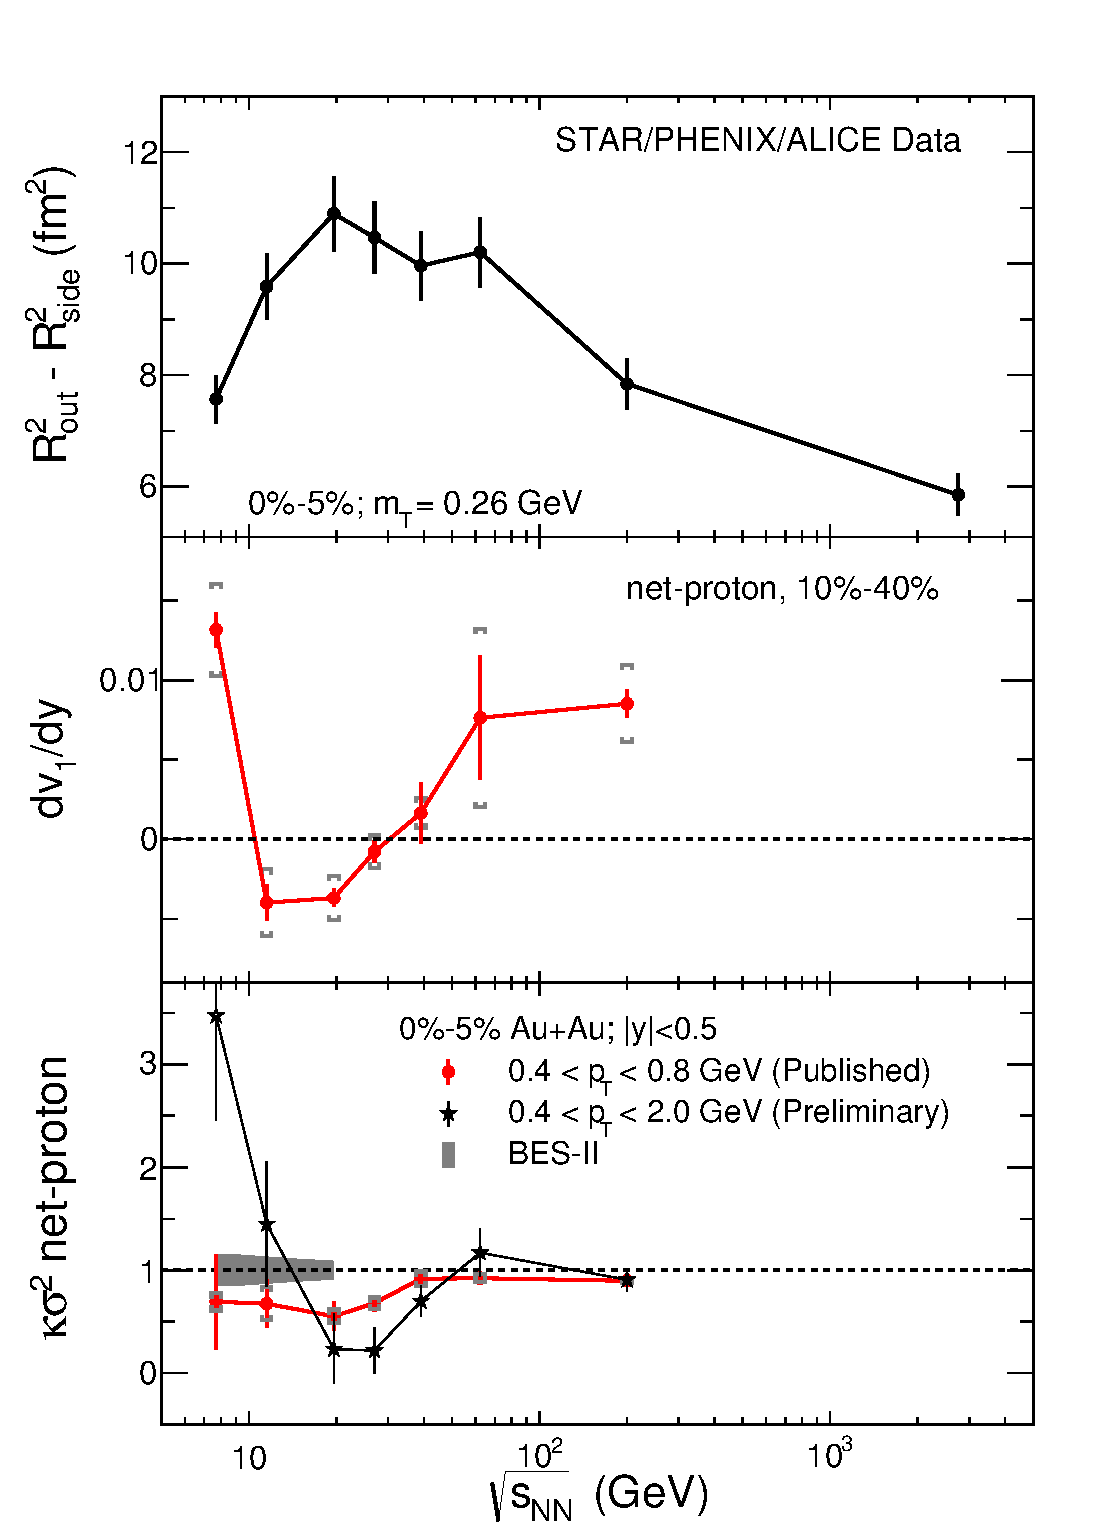
\includegraphics[width=0.7\textwidth]{fig/bes_compilation_prl_cpod.pdf}}
\caption[Observables showing non-monotonic behavior as a function of $\sqrt{s_\mathrm{NN}}$]{Three selected observables
  that all show interesting non-monotonic behavior as functions of collision energy around  $\sqrt{s_\mathrm{NN}}{\,\sim\,}15{-}40$\,GeV.  
    {\bf Top panel:}
  The difference 
  $R_{out}^{2}-R_{side}^{2}$
  between the squared radii
  in the outward and sidewards directions
  measured via two-pion interferometry
  vs. $\sqrt{s_{NN}}$ using STAR~\cite{Adamczyk:2014mxp}, PHENIX~\cite{Adare:2014qvs}, and 
  ALICE~\cite{Aamodt:2011mr}
  data. $R_{out}^{2}-R_{side}^{2}$, 
  reflects the lifetime of the
  collision fireball and was predicted~\cite{Rischke:1996em} to reach
  a maximum for collisions in which a hydrodynamic fluid forms at
  temperatures where the equation of state is softest.  
  {\bf Middle panel:} The rapidity-slope of the net proton directed flow $v_1$,
  $dv_1/dy$. This quantity is sensitive to early pressure gradients in
  the medium.  
  {\bf Bottom panel:} The kurtosis of the event-by-event
  distribution of the net proton (i.e. proton minus antiproton) number
  per unit of rapidity, normalized such that Poisson fluctuations give
  a value of $1$. In central collisions, published results in a
  limited kinematic range~\cite{Adamczyk:2013dal} show a drop below
  the Poisson baseline around $\sqrt{s_{NN}}=$27 and 19.6 GeV. New
  preliminary data over a larger $p_T$ range~\cite{CPODKurtosis},
  although at present still with substantial error bars, hint that the
  normalized kurtosis may, in fact, rise above 1 at lower
  $\sqrt{s_{NN}}$, as expected from critical fluctuations~\cite{Stephanov:2011pb}. 
  The grey band shows the much reduced
  uncertainties anticipated from BES-II in 2018-2019, for the 0-5\%
  most central collisions.}
\label{F-PD2}
%\vspace*{-5mm}
%}
%\end{minipage}
\vspace{-0.1in}
\end{center}
\end{figure}
%%%%%%%%%%%%%%%%%%%%%%%%%%%%%%%%%%%%%%%%%%%%%%%%%%%%%%%%%%%%%%
%



%%%%%%%%%%%%%%%%%%%%%%%%%%%%%%%%%
{\bf The need for BES-II and accompanying advances in theory}
%%%%%%%%%%%%%%%%%%%%%%%%%%%%%%%%%


Several observables from the
first phase of the RHIC Beam Energy Scan program (BES-I, introduced
in Section~\ref{Sec:BES})
exhibit interesting 
non-monotonic behavior as a function of collision energy,
and hence as a function of baryon number chemical potential $\mu_B$.
A selection of such measurements is shown in Figure~\ref{F-PD2}.  
At present, we await with considerable interest
the results from the final run in
the BES-I program at $\sqrt{s_{NN}}=14.5$\,GeV, where the data were taken only
a few months ago, since for a number of important observables the
measurements made previously at and below $\sqrt{s_{NN}}=19.6$\,GeV 
have quite
limited statistics. Nevertheless, it is already possible to see trends
and features in the data that provide compelling motivation 
for both a strong and concerted theoretical response aimed at quantitative
precision as well as for experimental measurements with much higher statistical precision at 
and below $\sqrt{s_{NN}}=19.6$\,GeV 
(i.e. at the largest achievable values of $\mu_B$)
that will be provided by the second phase of the Beam Energy Scan
program (BES-II) in 2018 and 2019. The goal of BES-II, as described
in more detail below, is to follow through in order to turn currently observed trends and
features into definitive scientific conclusions. As discussed in Section~\ref{Sec:RHICUpgrades}, 
the accelerator physicists at RHIC are planning a machine upgrade to
provide electron cooling to increase the beam luminosity at these
energies by about a factor of 10 \cite{BESII}. Targeted new detector
capabilities will also increase the sensitivity to the signals
described below in the BES-II campaign \cite{BESII}.

Experimental discovery of a first-order phase transition or a critical
point on the QCD phase diagram would be a landmark achievement. The
first goals of the BES program, however, have focused on obtaining a quantitative 
understanding of the properties of matter in the crossover region of the 
phase diagram as it changes with increasing $\mu_B$. Available tools
developed over the last few years now make a quantitative comparison
between theory and experiment tractable in the $\mu_B$-range
below any QCD critical point. Success in this effort, in and of itself, would
establish another major and lasting impact of the RHIC program. Questions
that can be addressed in this regime include quantitative study of the
onset of various signatures associated with the presence of
quark-gluon plasma and of the onset of chiral symmetry restoration as
one traverses the crossover region. Data now in hand from BES-I
provide key inputs and impetus toward this goal. Here we give four
examples, intended to be illustrative, of areas where a coherent
experimental and theoretical effort is expected to have substantial
impact on our understanding of QCD. In each case we note the
substantial impact expected from the additional measurements
anticipated during the BES-II:

{\bf 1.} The directed flow observable $dv_1/dy$ for net protons has been 
found to feature a dip as a function of collision energy (see middle panel 
in Figure~\ref{F-PD2}), with a minimum at energies somewhere between 
$\sqrt{s_{NN}}=11.5$ and 19.6\,GeV \cite{Adamczyk:2014ipa}. This has 
long been predicted in qualitative terms as a consequence of the 
softening of the equation of state in the transition region of the phase 
diagram \cite{Brachmann:1999mp,Stoecker:2004qu}. Several theoretical 
groups around the world have now begun hydrodynamic calculations with 
nonzero baryon density, deploying all the sophistication that has been
developed very recently in the analysis of higher energy collisions,
including initial fluctuations and a hadronic afterburner, in
applications to these lower energy collisions. These
hydrodynamic+hadronic cascade calculations will be used to compare the
$dv_1/dy$ data with equations of state in the crossover region of the
phase diagram obtained from lattice calculations via Taylor expansion
in $\mu_B/T$ \cite{Huovinen:2014woa}. This is a program where a
quantitative comparison, successful or not, will be of great interest,
since failure to describe the data could signal the presence of a
first-order phase transition. The precision of a comparison like this
will be substantially improved in 2018-19 when BES-II data will allow
$dv_1/dy$ to be measured for the first time with tightly specified
centrality; the statistics available in the BES-I data sets limit
present measurements to averages over collisions with widely varying
impact parameters \cite{Adamczyk:2014ipa}.

{\bf 2.} A second goal of the hydrodynamic calculations referred to
above will be to use identified particle BES-I $v_2$ data to map, in
quantitative terms, where and how hydrodynamics starts to break down
at lower collision energies, and where, to an increasing extent, $v_2$
develops during the hadron gas phase when viscosities are not small,
{\it i.e.}~where the contribution of the partonic phase to observed measures
of collectivity decreases in importance. A key future experimental
input to this program is the measurement of the elliptic flow $v_2$ of
the $\phi$-meson, which will be obtained with substantially greater
precision in the BES-II program. The first measurements of $v_2$ of
$\Omega$ baryons at these collision energies, also anticipated in
BES-II, will represent a further, substantial advance. Seeing $\phi$
mesons flowing like lighter mesons and $\Omega$ baryons flowing like
lighter baryons in collisions at a given energy would indicate that
the dominant contribution to the collective flow in those collisions
was generated during the partonic phase \cite{Abelev:2007rw}.

This component of the BES program, together with the following one,
will yield guidance as to what the lowest collision energies are at
which temperatures in the transition region of the phase diagram can
be explored. That is, they will tell us the largest value of  $\mu_B$ 
for which it will be
possible to use heavy-ion collisions, anywhere, to study matter in the
crossover region and search for a possible critical point.

{\bf 3.} Heavy-ion collisions at top RHIC energies and at the LHC have
now seen several experimental phenomena
\cite{Abelev:2009ac,Abelev:2012pa,Adamczyk:2013kcb} that may be
related to the chiral magnetic effect (CME
\cite{Fukushima:2008xe,Kharzeev:2010gr}, see Section~\ref{Sec:Exotica}). In
each case, alternative explanations are also being considered
\cite{Bzdak:2009fc,Pratt:2010zn}. One of the intriguing BES-I results
is that the three-particle correlations that are related to charge
separation across the reaction plane, possibly induced by the CME, are
clearly observable over most of the BES range but then seem to turn
off at $\sqrt{s_{NN}}=$ 7.7 GeV \cite{Adamczyk:2014mzf}, where the
elliptic flow $v_2$ is still robust. This is an indication that
$v_2$-induced backgrounds alone do not explain the observed
correlations. The observation that these three-particle correlations
disappear at the lowest energy could prove crucial to understanding
their origin and how they are related to the formation of QGP. On the
theoretical side, lattice QCD calculations probing the response of the
equation of state and transition temperature to the presence of
external magnetic fields~\cite{DElia:2010nq,Bali:2011qj,Bali:2014kia} are needed
to understand these signals.
Also necessary are hydrodynamic calculations incorporating magnetic fields and
chiral effects; these are being pursued by several groups, with
first results starting to appear~\cite{Hirono:2014oda}. On
the experimental side, higher statistics BES-II data will make it
possible to determine with much greater precision the $\sqrt{s_{NN}}$
at which this effect turns off and will also make it possible to
measure the (related but theoretically more robust) chiral magnetic
wave phenomenon~\cite{Kharzeev:2010gd,Burnier:2011bf}, which has also
been seen at top RHIC energy and at the LHC~\cite{Wang:2012qs,Belmont:2014lta}, 
and which should turn off below the
same $\sqrt{s_{NN}}$ where the CME-related observables
turn off, if these interpretations are correct.

{\bf 4.} Theoretical developments over the past decade have identified
specific event-by-event fluctuation observables most likely to be
enhanced in collisions that cool in the vicinity of the critical point
\cite{Stephanov:2008qz,Athanasiou:2010kw}. Higher moments of the
event-by-event distribution of the number of protons, or the net
proton number, are particularly sensitive 
\cite{Ejiri:2005wq,Athanasiou:2010kw,Karsch:2010ck}. STAR has now 
measured the first four moments (mean, variance, skewness and kurtosis) 
of the event-by-event distribution of net proton number and net charge at 
the BES-I energies \cite{Adamczyk:2013dal,Adamczyk:2014fia}. At the 
lowest collision energies, although the statistics are at present rather
limiting, there are interesting trends, including for example the drop in the
normalized kurtosis of the net-proton distribution at $\sqrt{s_{NN}}{\,=\,}27$
and 19.6 GeV (see bottom panel in Figure~\ref{F-PD2}). This drop in and 
of itself can be at least partially reproduced via prosaic effects captured 
in model calculations that do not include any critical point. Theoretical 
calculations of the contributions from critical fluctuations predict  
\cite{Stephanov:2011pb} that if the freezeout $\mu_B$ scans past a 
critical point as the beam energy is lowered, this kurtosis should first 
drop below its Poisson baseline and then rise above it. Both the drop 
and the rise should be largest in central collisions in which the 
quark-gluon plasma droplet is largest and therefore cools most slowly, 
allowing more time for critical fluctuations to develop~\cite{Berdnikov:1999ph}. 
A recent and still preliminary analysis~\cite{CPODKurtosis} 
that includes protons over a larger range in $p_T$ than measured before~\cite{Adamczyk:2013dal},
also shown in the bottom panel of 
Figure~\ref{F-PD2}, 
features a more substantial drop in the net proton kurtosis at $\sqrt{s_{NN}}$= 27 and 19.6 GeV
as well as intriguing hints of a rise above one at 
$\sqrt{s_{NN}}{\,=\,}11.5$ and  7.7\,GeV in central collisions, 
but the uncertainties are at present too 
large to draw conclusions. If this kurtosis does rise at $\sqrt{s_{NN}}$ 
values below 19.6 GeV, it would be difficult to understand in 
conventional terms and thus would be suggestive of a contribution 
from the fluctuations near a critical point. Determining whether this 
is so requires the higher statistics that BES-II will provide, as illustrated
by the grey band in the bottom panel of Figure~\ref{F-PD2}. 

The present data on moments of both the net proton number and the 
net charge at the higher BES-I energies are already very useful, as
they can be compared to lattice calculations of the Taylor expansions 
(in $\mu_B/T$) of the baryon number and charge susceptibilities~\cite{Karsch:2012wm}. 
First versions of this comparison have been
reported recently and are being used to provide an independent
determination of how the freeze-out values of $\mu_B$ and $T$ change
with collision energy~\cite{Bazavov:2012vg,Mukherjee:2013lsa,Borsanyi:2013hza,Borsanyi:2014ewa}. 
However, looking ahead, theoretical 
calculations will need to faithfully
account for the dynamical evolution of the medium formed in the
collision for a full quantitative exploitation of the experimental
data. For the higher statistics BES-II data on the net proton
kurtosis, skewness, and other fluctuation observables at low collision
energies to determine the location of the critical point on the phase
diagram of QCD, if one is discovered, or alternatively to reliably exclude its
existence within the experimentally accessible region of the phase
diagram, a substantial theoretical effort will be needed that couples
the sophisticated hydrodynamic calculations referred to above with a
fluctuating and dynamically evolving chiral  order parameter.

As the following fifth example illustrates, BES-II will also open the
door to measurements that were not yet accessible in the first phase
of the BES program:

%\begin{itemize}

%\item
{\bf 5.} Dileptons are unique penetrating probes with which to study
the chiral properties of hot and dense matter (see Section~\ref{Sec:EM}). The dielectron
invariant mass distributions measured in the BES-I (in data taken at
$\sqrt{s_{NN}}=$ 200, 62.4, 39 and 19.6 GeV; see Figure~\ref{fig:star-ee}) have shown that there is
a significant enhancement of low mass dileptons below 1 GeV relative
to a hadronic cocktail~\cite{Huck:2014mfa}. The data so far are qualitatively
consistent with a model in which hadron properties are modified in the
medium and there is a partonic contribution as
well~\cite{Rapp:2009yu}. However, data at lower energies with higher
statistics are crucial in order to test the predicted strong
dependence of dilepton yields on baryon density and draw firm
conclusions. The dilepton measurements at and below
$\sqrt{s_{NN}}{\,=\,}19.6$\,GeV that BES-II will provide will yield a
qualitatively new understanding of the chiral properties of QCD matter
with significant baryon density. There are two interesting dilepton
mass windows to be studied at BES-II: the low mass window (300 MeV --
700 MeV) and the high mass window (800 MeV -- 1.5 GeV). The former
will provide indirect information on chiral symmetry restoration via
the interaction of vector mesons with (excited) baryons, while the
latter will probe chiral restoration directly via the mixing between
vector and axial-vector mesons in the hot and dense environment.

%\end{itemize}

Each of these five examples makes it clear that in order to maximize
the physics outcome from BES-I and BES-II, a coherent effort between
experimentalists and theorists working on QCD at nonzero $T$ and
$\mu_B$ is essential.
%and must be organized and supported. 
Indeed,
there has been considerable progress in lattice QCD recently on the
calculation of various QCD susceptibilities
\cite{Borsanyi:2011sw,Bazavov:2012jq} and the QCD equation of state in
the regime where $\mu_B$ is nonzero but sufficiently small compared to
$3\,T_c$ \cite{Borsanyi:2012cr,Hegde:2014wga}. These lattice
calculations provide the necessary inputs for extending 
the kind of sophisticated hydrodynamic calculations (including
initial fluctuations and a late stage hadron cascade) that have been
developed over the past few years to nonzero $\mu_B$. For some purposes, these
calculations additionally require coupling to a fluctuating and evolving
chiral order parameter.
%
In concert, such developments will provide the critical tools for
obtaining from BES-I and BES-II data answers to fundamental questions
about the phases, the crossover, and perhaps the critical point and
first-order transition, in the QCD phase diagram. 


The examples that we have sketched show that BES data,
at present and in the future from BES-II, 
together with the concerted theoretical response that present
data motivates will yield quantitative
understanding of the properties of QCD matter in the crossover region
where QGP turns into hadrons. 
If there is a critical
point with $\mu_B<400$~MeV, BES-II data on fluctuation and flow 
observables together with the theoretical
tools now being developed should yield quantitative evidence for its
presence.  
%
The span in $T$ and $\mu_B$ that the flexibility of RHIC
makes accessible, along with the technical advantages of
measuring fluctuation observables at a collider mentioned in Section~\ref{Sec:CP},
together with the 
recent and planned
detector and facility upgrades (low energy electron cooling in particular), 
mean that RHIC is uniquely positioned in the world 
to discover a critical point in the
QCD phase diagram if Nature has put this landmark in the
experimentally accessible region. Late in the decade, the FAIR
facility at GSI\cite{FAIR} will extend this search to even higher $\mu_B$ if its
collision energies continue to produce matter at the requisite
temperatures.


\subsection{Hard Probes of the Quark-Gluon Plasma}
\label{Sec:HardProbes}

High transverse momentum single hadrons, fully reconstructed jets,
open heavy flavor and heavy quarkonia provide information about the
strongly coupled QGP that complements the information provided by the
bulk and collective observables of the soft sector.  The higher
momentum and mass scales of these hard probes drive their production
to the earliest times in the collision; these same properties imply
that these probes don't completely thermalize during the evolution of
the produced medium.  The information imprinted on hard probes by QGP
production mechanisms and its later dynamics can therefore survive
into final state observables, making them uniquely valuable as
investigative tools of the complex emergent physics of the QGP.
However, accessing these very positive attributes of hard probes is
complicated in many cases by small production cross sections or the
need for specialized techniques and detectors.

In this section we first outline the future of jet studies over the
next decade, enabled by major developments in the RHIC and LHC
accelerator facilities and experiments described in
\ref{Sec:FacilitiesFuture}.  After that, we focus on the coming
prospects for open heavy flavor and heavy quarkonia measurements.

\subsubsection{Overview}

Previous studies at RHIC and the LHC have clearly demonstrated the ability 
to reconstruct jet observables in the high multiplicity heavy ion environment. 
Comparisons of hadronic and jet-based measurements to model calculations 
in a perturbative QCD framework have allowed the extraction of the QGP transport coefficient  \qhat\
with an uncertainty of about 50\%. Full jet 
measurements have demonstrated the modification of the dijet and photon-jet
momentum balance due to energy loss in the QGP, and have provided 
the first look at the modification of the jet structure itself due to 
interactions of the hard probe with the medium. These studies demonstrate the 
transport of energy from the jet core to low transverse momenta, close 
to thermal momentum scales, and away from the jet axis towards 
large angles far outside of the typical jet cone definition.

Future jet-based studies, built on the achievements at RHIC and the LHC, will 
address fundamental questions about the nature of QGP. These include 
precise measurements of QGP transport coefficients as a function of 
temperature, a detailed characterization of the QGP response to the 
parton energy loss and studies of the modification the jet angular 
and momentum structure as a function of angular and momentum scale. 
In combination, the goal of these studies is to determine the 
microscopic (or quasi-particle) nature of QGP 
and to understand how the macroscopic QGP liquid emerges from the 
underlying QCD degrees of freedom by probing the QGP dynamics over a wide range of length scales, see Figure\ \ref{Fig:HardProbesFuture} for a graphical representation.

This program will be enabled by the evolution of the RHIC and LHC 
accelerator facilities, upgrades to the existing experiments and the 
construction of sPHENIX, a state-of-the-art jet detector at RHIC. In 
parallel, experiment/theory collaborations will be strengthened 
and expanded, to fully utilize the increased precision and range of 
experimental observables. 

\begin{figure}[t]
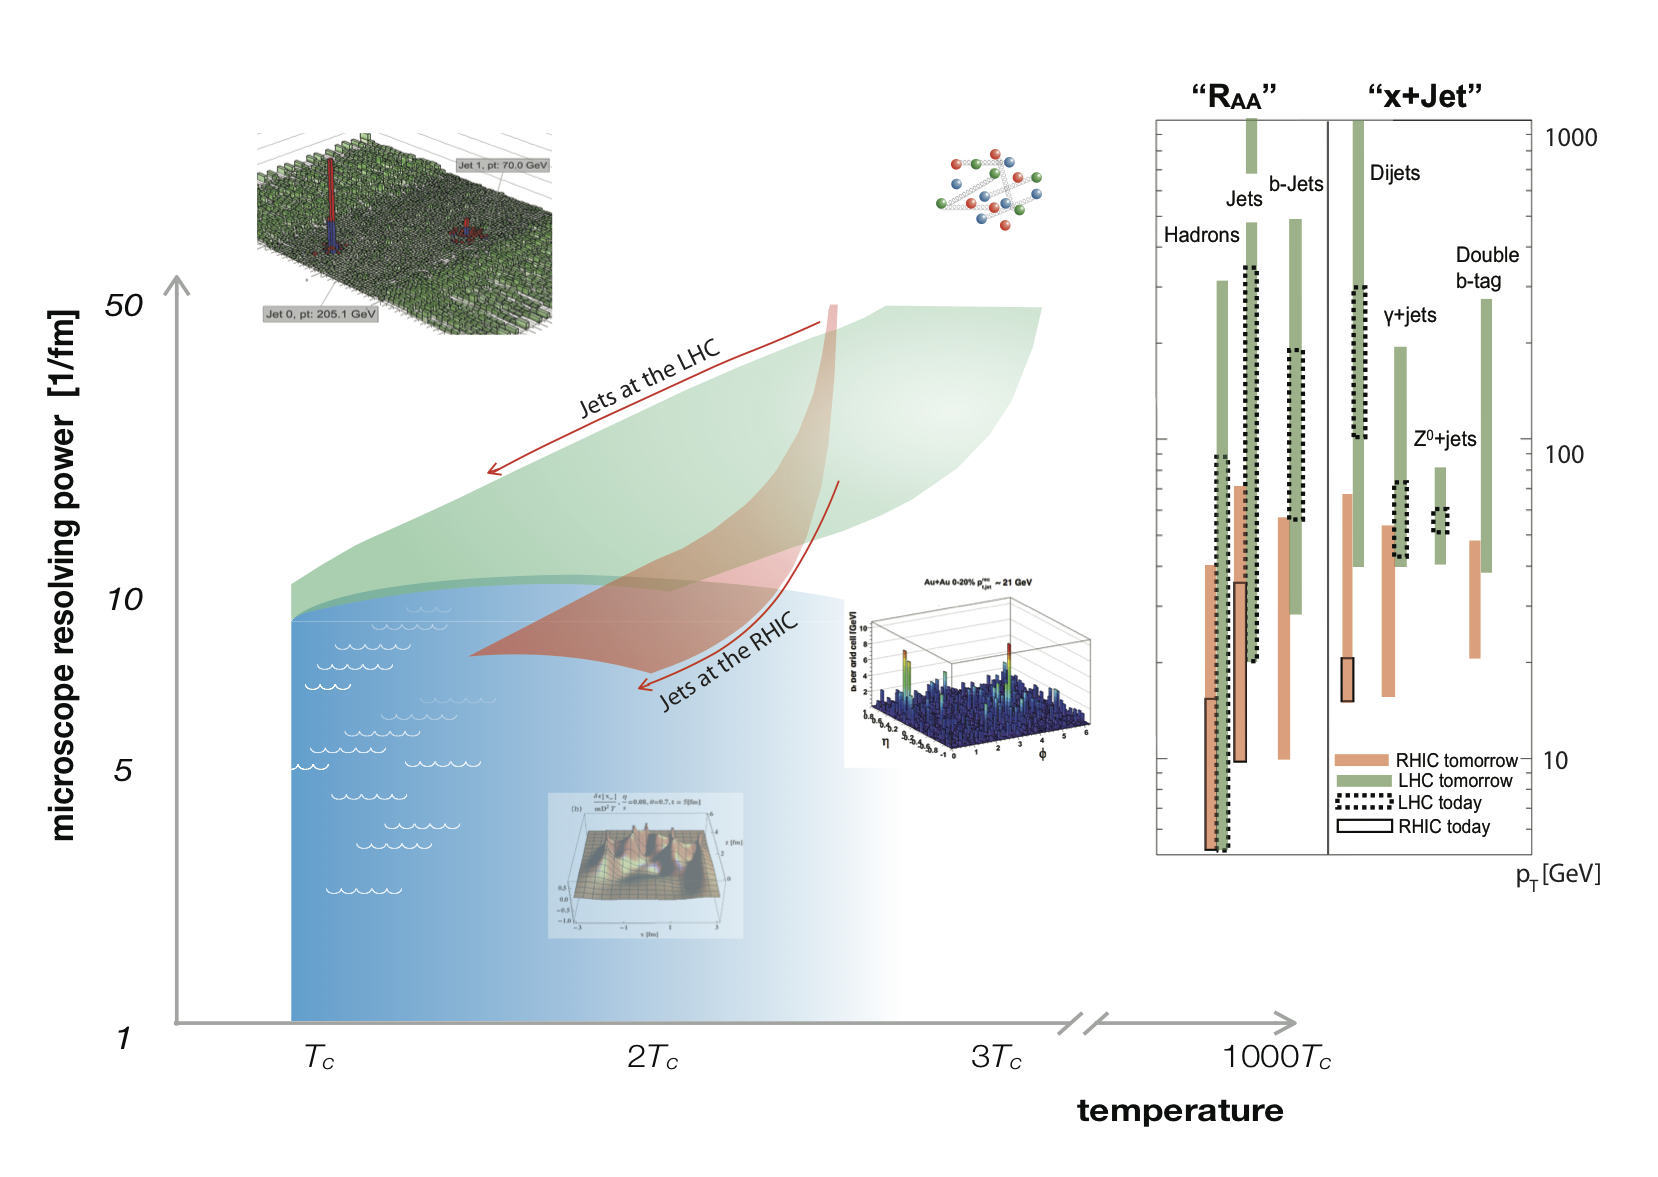
\includegraphics[width=1.05\textwidth]{fig/HardProbesFuture}
\caption[Graphical representation of a future physics goal]{Graphical representation of the future physics goal: Hard scattered partons at the LHC and at RHIC evolve through splittings and interaction with the medium, providing sensitivity to QGP dynamics over a wide range of length scales. The kinematic reach of future RHIC and LHC jet observables and their important kinematic overlap, enabled by new instrumentation at RHIC, is shown in an artist rendering.}
\label{Fig:HardProbesFuture}
\end{figure}

\subsubsection{Future jet physics capabilities at RHIC and LHC}
\label{Sec:FutureJetCapabilities}

Section~\ref{Sec:FacilitiesFuture} has provided an outline of the RHIC and LHC
accelerator and experiment upgrade plans. These upgrades benefit jet physics studies
at the two facilities in three major ways:
\begin{enumerate}
\item The statistical precision and kinematic reach for commonly used jet physics observables
is vastly increased, as shown in \ref{Fig:HardProbesFuture}). For single charged hadrons and reconstructed jets, the \pT\ reach will be 
extended by a factor of 2--3, up to 40~GeV for hadrons and 70~GeV for jets at RHIC (see Figure\ \ref{fig:AAphysics_projections}) and 
300~GeV and 1~TeV, respectively, at LHC. The increased lever arm will be crucial in further improving
the extraction of e.g.\ the \qhat\ coefficient from model comparisons. Equally importantly, 
the larger data sets will allow a more detailed determination of \qhat\ as a function
of path length and medium conditions, e.g.\ in very peripheral collisions in the two 
energy regimes.

\item Beyond increasing the kinematic range and statistical precision for 
current ``workhorse'' measurements, the combination of the increased luminosity at RHIC and LHC, 
increased LHC collision energy and the experiment upgrades will move 
the focus of experimental and theoretical studies to rare, highly specific
observables. Key examples are measurements of isolated photon + jet 
correlations at RHIC and LHC, as well as $Z^0$+jet correlations at LHC. 
As a benchmark, the number of recorded photon+jet events at LHC 
with $\ptg > 60$~GeV is expected to reach more than $3 \times 10^5$, compared
to about 3000 in the Run I data sets. Using the photon tag, the initial
energy of the scattered parton is determined on an event-by-event basis to about 15\%.
The photon tag also identifies the partons as quarks and provides their 
initial direction. Furthermore, the comparison of photon+jet events 
at RHIC and the LHC allows the selection of nearly identical initial 
hard scattering configurations embedded in different initial medium conditions
in terms of temperature and energy density (see Figure\ \ref{Fig:HardProbesFuture}). As jets and the medium co-evolve 
from their initial virtuality and conditions to final state hadrons, 
the comparison of various observables between the RHIC and LHC events
will provide key insights into the temperature dependence of the jet-medium
interactions. Future measurements enabled by this program include the 
absolute quark energy loss
as a function of quark energy and path length, modifications of the 
jet momentum and angular structure and the large angle momentum flow
and medium response as a function of event-by-event jet energy loss.
\item Finally, the very high statistics jet samples to be collected at the LHC and 
with a future state-of-the-art jet detector at RHIC will allow analyses based on 
a new generation of jet shape observables. There is intense activity
in the development of generalized jet structure variables at the LHC to maximize
the efficiency of discovery measurements by improving quark/gluon
discrimination and the tagging of boosted objects. Heavy ion studies 
of the modification of the jet momentum and angular structure through 
medium interactions will benefit greatly from these developments.
Present measurements at the LHC have shown the jet structure to be modified 
both within a typical jet cone size (e.g. $R = 0.5$) and beyond, with
the fragmentation products inside the cone shifted towards 
lower $\pt$ and larger angles and an associated transport of most of the ``lost''
jet energy outside of the typical jet cone size. First results 
at RHIC, probing different medium conditions, indicate similarities
in the modifications of the jet momentum structure, but possible
differences in the angular modifications. Using common, well-calibrated
jet shape observables at RHIC and the LHC in different regimes of 
medium conditions will be critical in relating the observed 
modifications to the fundamental properties of the QGP,
in extracting the temperature dependence of QGP transport coefficients
and ultimately in understanding the nature of the medium in the vicinity
of the phase transition and at temperatures much larger than $T_C$.

\end{enumerate}

\subsubsection{Future jet probes of the QGP}
\label{Sec:FutureJetProbes}

The combination of large increases in delivered luminosity over the next
decade, upgrades to the existing LHC detectors and the construction
of a state-of-the-art jet detector at RHIC will enable a coherent 
physics program employing well-calibrated common observables to
study jet modifications and jet-medium interactions over a wide 
range of medium conditions created at RHIC and the LHC, as shown
schematically in Figure\ \ref{Fig:HardProbesFuture}.
Together, RHIC and the LHC will provide a physics program that includes
a precision extraction
of QGP transport coefficients related to jet-medium interactions.
Even more importantly, this program will employ jets as a tool to understand how the 
observed strongly coupled (liquid) nature of the QGP arises from the 
underlying QCD micro-physics by probing the QGP dynamics over a wide range of length scales (see Figure\ \ref{Fig:HardProbesFuture}). 
By conducting these investigations we will move from observing what the properties
of QGP are to understanding how these properties 
arise from the underlying gauge theory.
%%%%%%%%%%%%%%%%%%%%
\pagebreak
%%%%%%%%%%%%%%%%%%%%

\begin{figure}
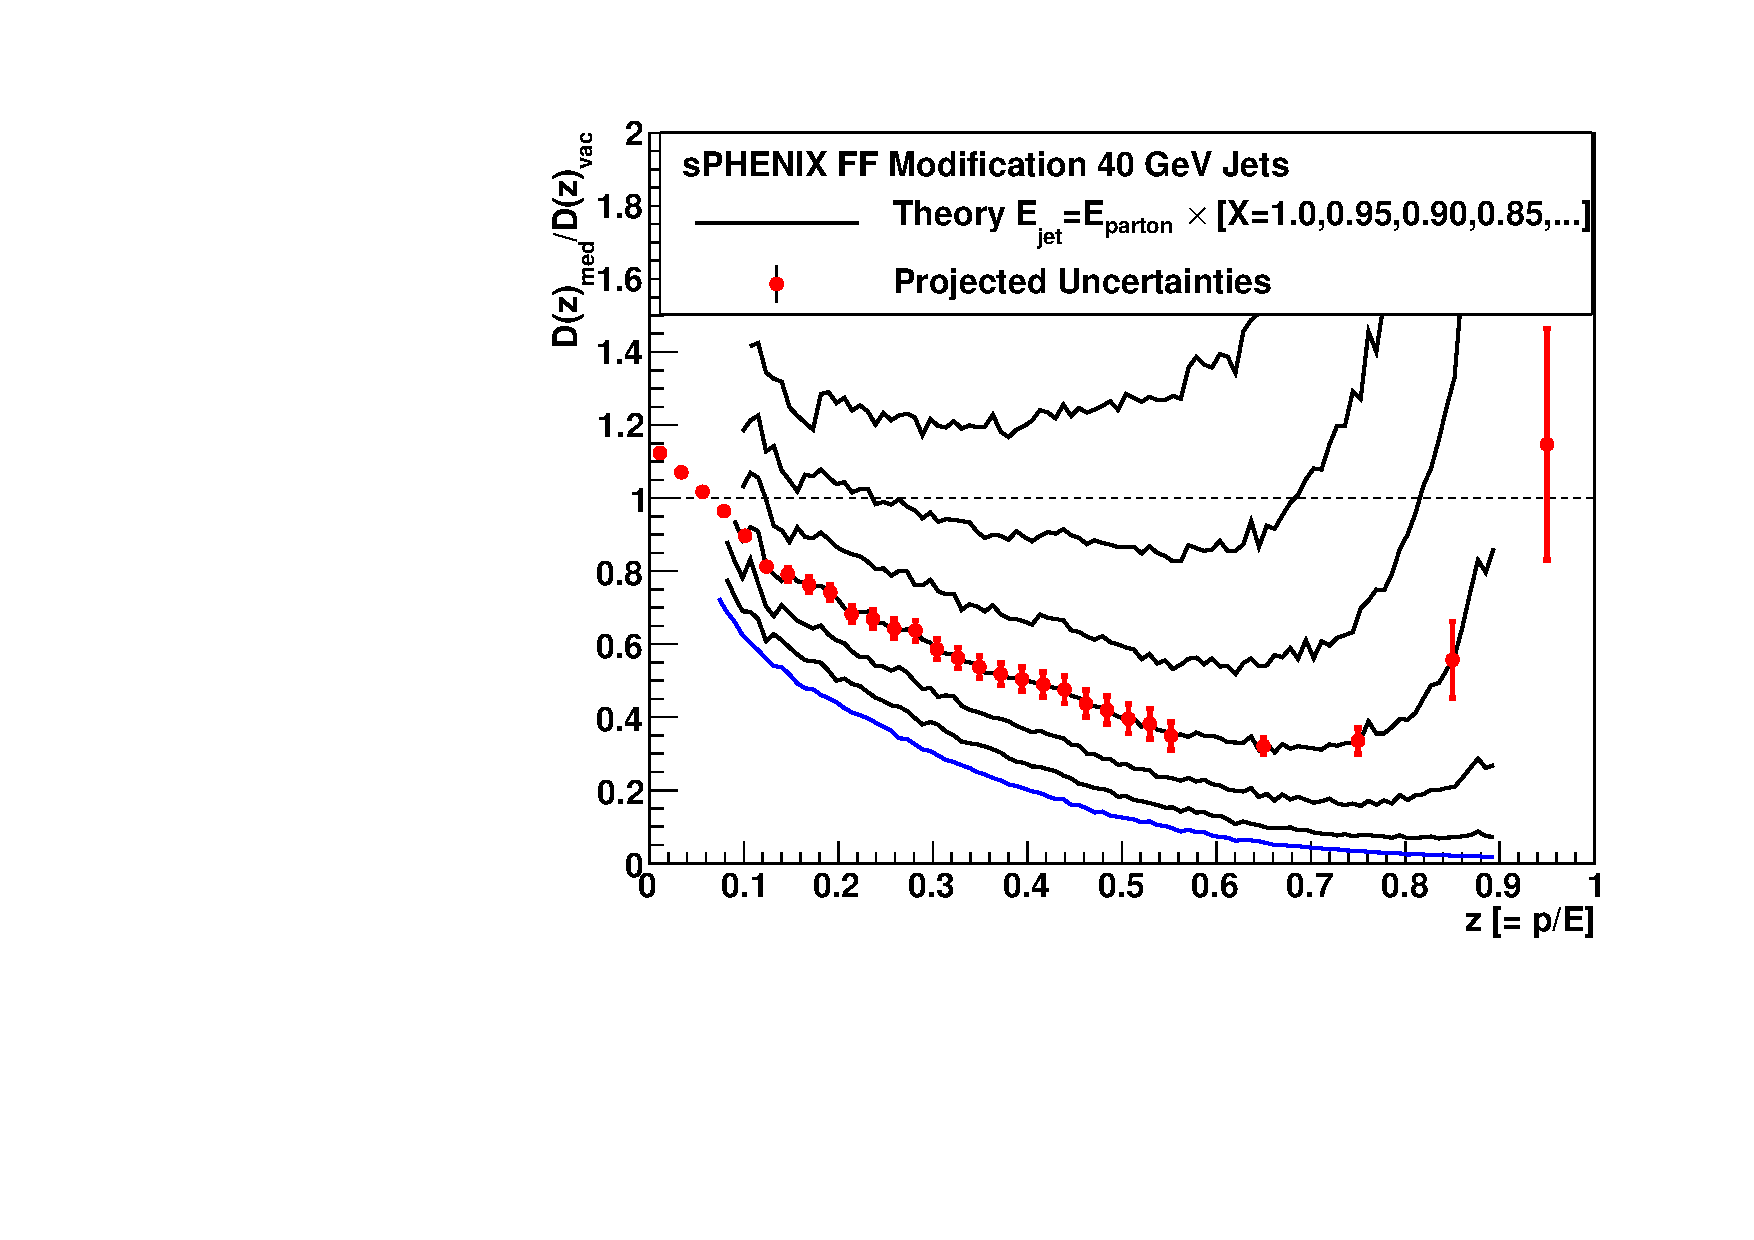
\includegraphics[width=0.9\textwidth]{fig/figure_ffmodification.pdf}
\caption[Projected sPHENIX statistical uncertainties on modified fragmentation functions]{Modified fragmentation function $D(z)$ in the medium\cite{Armesto:2007dt} expressed as the ratio of the modified $D(z)$ to that assuming vacuum fragmentation. The different black curves show the results of different assumptions for the fraction $X$ of the parton energy retained in the jet cone, with the original prediction corresponding to $X = 1.0$ shown as the lower blue curve. The projected statistical uncertainties are those achievable with sPHENIX for 22 weeks and 10 weeks of Au+Au and p+p data-taking, shown superimposed on the curve for $X = 0.85$. }
\label{Fig:sPHENIXfragfn}
\end{figure}
In detail, this future program includes:
\begin{enumerate}
\item Increased precision in extracting the average \qhat\ and \ehat\ 
transport coefficients, leading to a determination of their scale, energy and temperature dependence.
\item Combined global analysis of multiple observables at RHIC and the LHC 
to extract the temperature dependence of transport coefficients. Both
the RHIC and LHC final states represent an integral of jet-medium
interactions over the evolution of both the jet and the medium from initial
to final state. To disentangle the temperature dependence from
this evolution it will be essential to deploy directly comparable 
observables (theoretically and experimentally) in different 
QGP temperature regimes, in particular with respect to the fraction
of their evolution spend in the vicinity to the phase transition
region. Only a combined effort at RHIC and LHC can address this 
question.
\item Using increased systematic and statistical precision afforded
by new probes (e.g. photon-jet) to identity the medium response to
the modified jet radiation and further elucidate the liquid nature 
of the medium in its response to local perturbations
\item Using precision measurements of modifications of the jet structure 
in angular and momentum space to characterize the microscopic structure 
of the QGP. Jet probes here serve to perform experiments analogous to
Rutherford or deep-inelastic scattering off effective QGP constituents or 
quasi-particles. 
Perhaps the most straightforward signal is the modification of the 
jet fragmentation function $D(z)$, where $z = p/E$ is the momentum fraction 
of a single-particle of momentum $p$ in a jet of energy $E$. 
Other interesting observables include both potential modifications 
to the back-to-back jet scattering distributions, as well as modifications
of the intra-jet angular structure. For the latter, the correlated 
angular and momentum evolution of the jet from the initial scattering 
to the final hadronic structure probes probes a wide
range of scales, opening a window to interactions of jet 
and QGP constituents in between vacuum-like and in-medium cascade 
regimes. To pin down the physics of this intermediate window, 
systematic variations of both the jet conditions 
and medium conditions and dynamics are necessary. Combining RHIC and LHC 
measurements will allow control over initial density and temperature 
(in particular in respect to their vicinity to the critical temperature) 
and expansion dynamics of the system. The different energy regimes and 
tagging of particular initial states (photon+jet, $b$-tagged jets, 
multi-jet events) will allow selection of different or common 
jet populations in relation to different medium conditions. Success in 
this long-term endeavor will require a global analysis of 
a diverse set of RHIC and LHC data in an improved, well controlled
theoretical framework that makes explicit contact with the experimental observables.
\end{enumerate}


\subsubsection{Future challenges in the theory of jet modification}
\label{Sec:FutureJetTheoryChallenges}

In the period subsequent to the 2007 long range plan, there has been a major advance in the theoretical description 
of jet modifications in a dense medium. The ability of experiments both at RHIC and LHC to study full jet modification and 
energy flow with respect to the jet axis has led to the evolution from formalisms focused only on the leading particle towards full jet analyses tools.
Primarily, this has led to the ongoing development of several Monte-Carlo codes: YaJEM~\cite{Renk:2008pp,Renk:2010zx}, JEWEL~\cite{Zapp:2008gi}, MARTINI~\cite{Schenke:2009gb}, Q-PYTHIA~\cite{Armesto:2009fj}, PYQUEN~\cite{Lokhtin:2011qq}, and MATTER~\cite{Majumder:2013re}. While most of these routines are based on weak coupling, there is also a recently developed generator that is based on a hybrid strong and weak coupling approach~\cite{Casalderrey-Solana:2014bpa}. 

All of these approaches are based on one of the established analytical formalisms, and as such, apply to slightly different epochs in the lifespan of a hard jet in a dense medium. As a jet emanates from a hard interaction, it is far off its mass shell, at such hard scales that the jet probes the medium at extremely short distances characterized by its high-$Q^{2}$ 
structure of a dilute gas of partons. In this regime, it is expected that the parton's interactions with the medium are
dominated by radiation of gluons over elastic scattering processes.  
As the virtuality of the partons within a jet begins to drop, different parts of the jet enter different regimes.
The very energetic jet fragments undergo several scatterings per emission in which the multiple scattering prevents their virtuality from falling
below $\hat{q} \tau$, where $\tau$ is the lifetime of 
the parton.
As a result, those hard partons remain weakly coupled with the medium. 
The less energetic partons in the shower decrease in virtuality to the scale of the medium 
(of the order of the local temperature) and become strongly coupled. 
Currently most of the Monte Carlo descriptions apply to only one of these regimes, under the assumption that such a regime dominates the measured observables (with varying approximations regarding the medium). 
Nonetheless, several of these event generators have been tested against a variety of observables, 
such as jet $R_{AA}$,
dijet energy and angular imbalance, 
intra-jet hadron distribution and jet shapes~\cite{Renk:2013rla,Renk:2012cb,Ramos:2014mba,Zapp:2012ak,Young:2012dv,Majumder:2013re}. 
One of the outstanding challenges in this field will be the development of a generator that smoothly interpolates between the various regimes of jet quenching while incorporating a fluctuating medium simulated by an event-by-event viscous fluid dynamical simulation. This will be followed by rigorous testing and validation against all available 
jet data. 


Full jet reconstruction, however, involves more than simply a perturbative redistribution of the energy within a jet cone.
Rather, as the energy is deposited within an evolving medium it thermalizes and forms a source of energy and momentum current for the fluid dynamical evolution of the medium. 
A significant fraction of the this energy is carried away from the jet at large angles, with the remainder found 
within the reconstructed jet cone. To date only initial efforts have been made to understand the dynamics of energy deposition and redistribution 
within a fluid medium~\cite{Neufeld:2009ep,Qin:2009uh}, and this remains an open issue. 
In addition to this question of energy redistribution at the medium scale, another outstanding question is the distribution of radiation at the perturbative scale. The ordering of radiation from a hard parton in vacuum is well established, however its modification in the medium is still an open question. There now exist two separate calculations, one in the radiation dominated regime~\cite{Fickinger:2013xwa} which shows no ordering, and one in the 
scattering dominated regime~\cite{Armesto:2011ir}, which shows anti-angular ordering. A resolution of these issues at NLO remains one of the major opportunities in the theory of 
pQCD energy loss. It may indeed turn out that a full understanding of this problem leads to the development of an effective theory of jet modification in dense matter. To date, 
great strides have been made in modifying Soft Collinear Effective Theory (SCET)~\cite{Bauer:2000yr,Bauer:2001yt,Bauer:2002nz} by the addition of off-shell gluon modes with momenta transverse to the collinear modes within a hard jet. 
This modified version of SCET has been uses to calculate the 
propagation, scattering and emission from hard partons in a dense medium~\cite{Idilbi:2008vm, DEramo:2010ak,Ovanesyan:2011xy}. Extending this beyond the radiation dominated regime to the multiple scattering regime remains a future goal. Several model calculations~\cite{CasalderreySolana:2011rq,Qin:2010mn} have already laid the groundwork for what a fully developed jet modification theory should look like. 


Developing in parallel with the theoretical description of parton showers in a dense medium is the improved description of transport coefficients, which are the actual measurable quantities that describe the medium probed by hard jets. A great deal of work has gone into determining the temperature dependence of the transverse diffusion coefficient $\hat{q}$. 
More recently, efforts have been made to determine the longitudinal energy loss coefficient $\hat{e}$. 
While light flavor energy loss is known to be weakly dependent on $\hat{e}$, this is not the case for 
heavy flavors. 
Significant theoretical activity now focuses on determining the dynamics of heavy flavor energy loss 
and the sensitivity of these and other heavy flavor observables
to $\hat{e}$~\cite{Qin:2009gw,Djordjevic:2013pba,Abir:2014sxa}. 
Efforts to extend this to $b-$tagged jets are also being carried out~\cite{Huang:2013vaa}. 
Future developments in the theory of heavy flavor dynamics in the medium serve not only as a consistency check for the pQCD based formalism of jet modification, but also provide the 
primary means to determine the drag coefficient $\hat{e}$.

While the dependencies of the transport coefficients on temperature reveal the dynamics of the medium as seen by the jet, they also depend on the scale and energy of the jet. 
Recently there has been a series of developments to quantify this scale and energy dependence of transport coefficients by carrying out NLO calculations of these coefficients, 
most notably of $\hat{q}$. Several calculations, once again performed in different regimes of jet quenching, have obtained rather different dependencies on energy and 
scale~\cite{Liou:2013qya,Kang:2013raa,Blaizot:2014bha,Iancu:2014kga}. Much theoretical effort is currently being devoted to a resolution of these differences. 
In all of the current jet quenching calculations, either of leading particles or of full jets, the normalization of the transport coefficients is determined
empirically by fitting to one data set. 
%This situation will remain 
%even after all issues with renormalization have been settled.
While this emphasizes the absolute requirement of parallel theoretical and experimental investigations,
it also demonstrates that the current calculations of jet modifications do not result directly from the QCD Lagrangian. In an effort to 
resolve this, several groups have considered the possibility of evaluating such coefficients 
on the lattice~\cite{Majumder:2012sh,Panero:2013pla,Ji:2013dva}. These represent 
extremely difficult calculations which, however, hold the promise of determining the transport coefficients with no input other than the local temperature. 
Future calculations of transport coefficients on the lattice, combined with calculations of the 
scale and energy dependence described above will allow for a rigorous and first principles test of the entire formalism of jet modification.



\subsubsection{Future Quarkonia measurements at RHIC and the LHC}
\label{Sec:FutureQuarkonia}

%\begin{figure}[!pht]
%   \centering
%   \begin{subfigure}[b]{0.72\textwidth}
%      \includegraphics[width=0.9\textwidth]{fig/upsilon_mass_subtracted_0_10pc_10Bevts}
%       \caption{The di-electron invariant mass distribution  for 0--10\% central \AuAu\ events after 
%                      the combinatorial background has been removed by subtracting all like-sign pairs.}
%        \label{Fig:upsilon_auau_0-10pc}
%    \end{subfigure}
%    
%    \begin{subfigure}[b]{0.72\textwidth}
%        \includegraphics[width=0.9\textwidth]{fig/upsilon_raa_10pc_bins_100Bevts}
%        \caption{ Estimate of the statistical precision of a measurement of the
%                       $\Upsilon$ states assuming that the measured $R_{AA}$ is equal to the results of a recent theory
%                      calculation~\cite{Strickland:2011aa} }
%         \label{Fig:upsilon_raa}
%    \end{subfigure}
%
%    \caption{Projected quarkonia results from a 10 week \AuAu\ run with sPHENIX.}
%\end{figure}

\begin{figure}[!pht]
  \centering
      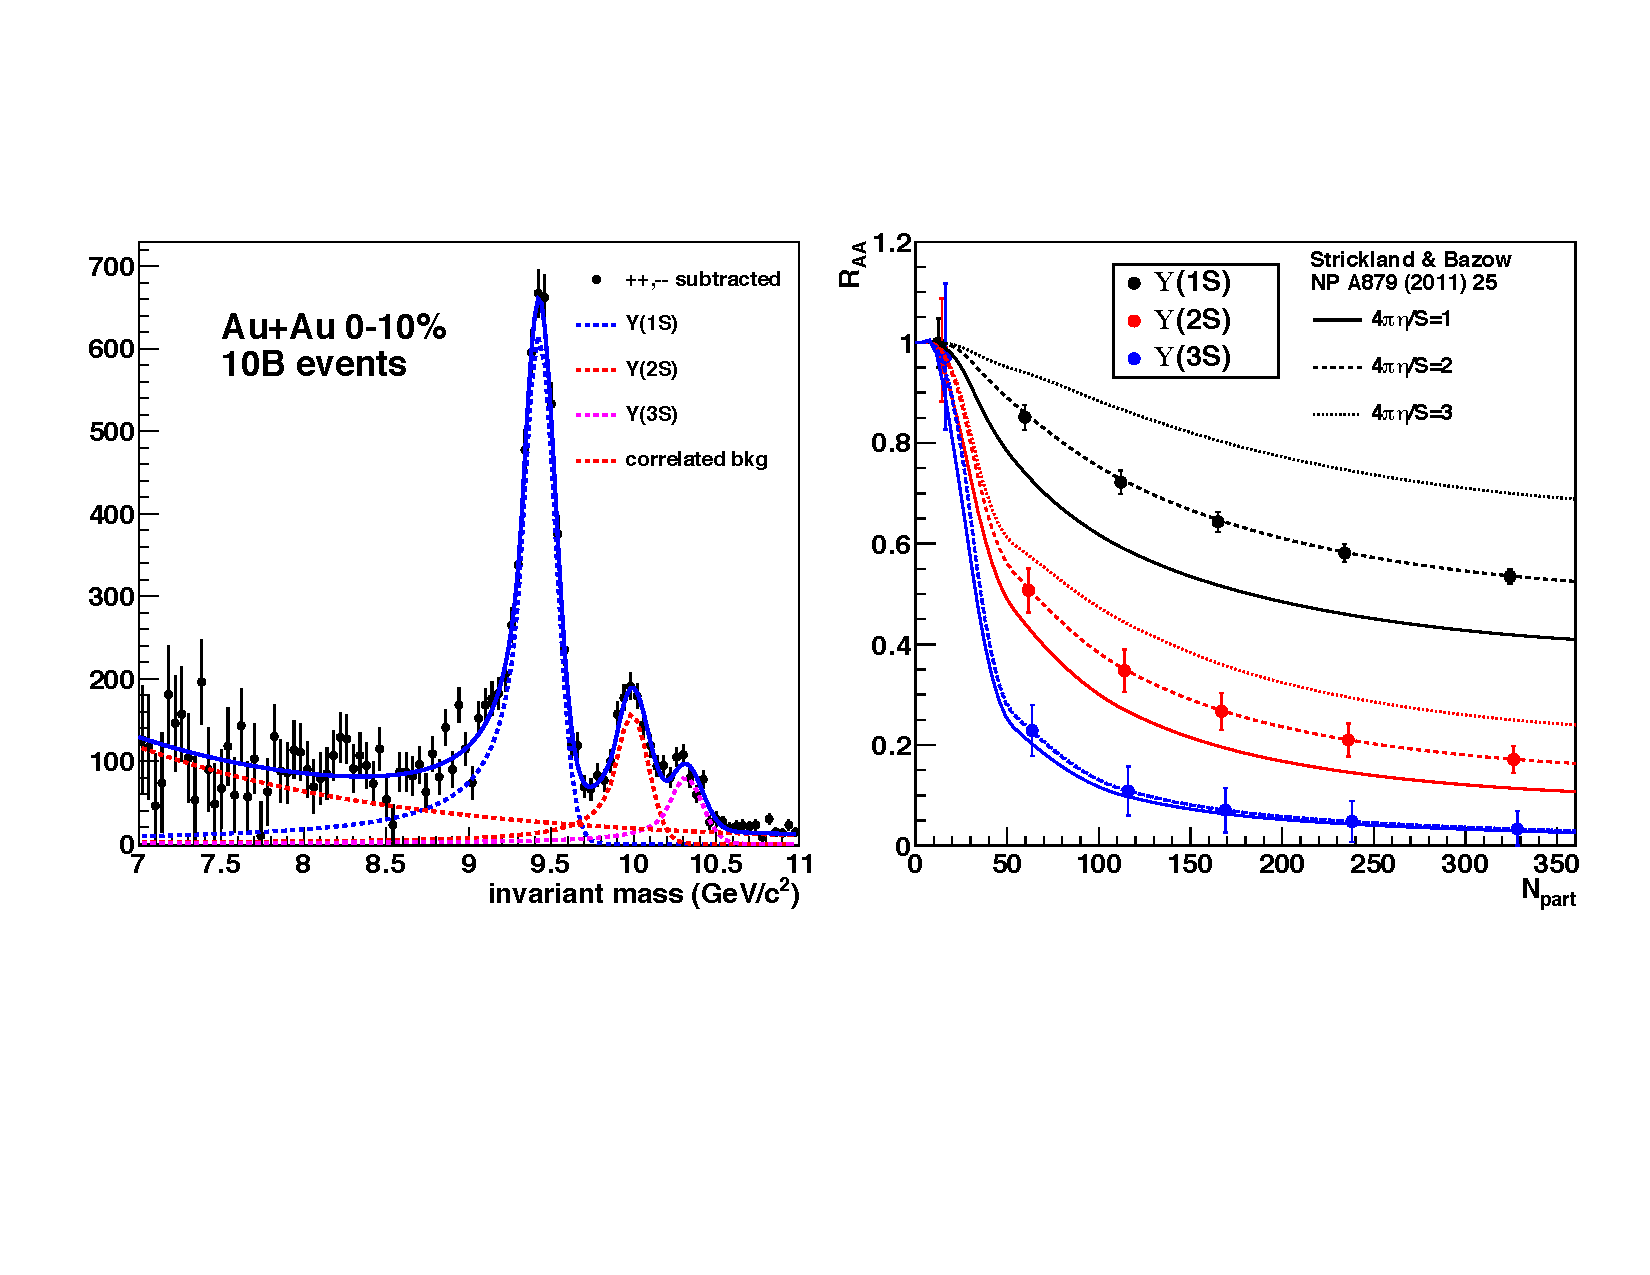
\includegraphics[width=\textwidth]{fig/upsilon_combined}
      \caption[Projected quarkonia results from a 20 week \AuAu\ run
        with sPHENIX]{Projected quarkonia results from a 20 week \AuAu\ run
        with sPHENIX.  (left) The di-electron invariant mass
        distribution for 0--10\% central \AuAu\ events after the
        combinatorial background has been removed by subtracting all
        like-sign pairs. (right) Estimate of the statistical
        precision of a measurement of the $\Upsilon$ states assuming
        that the measured $R_{AA}$ is equal to the results of a
        recent theory calculation~\cite{Strickland:2011aa}.}
\label{Fig:upsilon_auau_0-10pc}
\label{Fig:upsilon_raa}
\end{figure}

In addition to the jet capabilities added at RHIC by the sPHENIX detector upgrade, 
outlined in Section~\ref{Sec:FacilitiesFuture}, high precision
measurements of the modification of the $\Upsilon(1S)$, $\Upsilon(2S)$ and $\Upsilon(3S)$
states in A+A and $p$+A collisions will also be provided by sPHENIX. The key features 
of the upgrade that enable this are:

\begin{itemize}

\item The 1.5 T magnetic field of the Babar magnet, combined with precise tracking, will 
provide 100 MeV mass resolution for measurements of $\Upsilon \rightarrow e^+e^-$ decays
at mid rapidity.

\item Good signal to background performance is obtained by using low mass tracking to limit 
radiative losses for electron tracks and the Electromagnetic and Hadronic calorimeters to 
reject combinatoric background from charged hadrons.

\item Increased RHIC luminosity combined with the large acceptance of sPHENIX
and long RHIC running times provide the statistical precision for the $\Upsilon$ measurements at RHIC that will
tightly constrain theoretical models of the modification. These measurements will 
complement similar high precision measurements at higher temperature from LHC 
experiments that will be available on a similar time scale (i.e. by the end of LHC Run 3) 
due to LHC machine and detector upgrades, and accumulated luminosity.

\end{itemize}

Critical variables to manipulate when probing the QGP are the temperature of
the QGP and the length scale probed in the medium. For this reason, measurements 
at two widely different temperatures of the three Upsilon states, which span a large range of 
binding energies and sizes, are ideal. However for comparisons between data at RHIC and the LHC
 to be effective, high precision is required at both facilities.

The planned program of measurements at RHIC starting in 2021 includes \pp\,
\pAu\ and \AuAu\ measurements. A very important feature for $\Upsilon$ 
measurements with sPHENIX is that the increases in \pp\ luminosity at RHIC will permit a
measurement of the \pp\ reference cross section having similar precision to that which can be
attained in \AuAu\ and \pAu\ collisions. The projected invariant mass spectrum for central collisions
from a 10 week \AuAu\ run is shown in Figure~\ref{Fig:upsilon_auau_0-10pc}. This spectrum is shown
after the combinatorial background has been subtracted, and assumes no modification of the yields relative
to \pp\ collisions. 


The projected statistical precision for measuring the nuclear suppression factor $R_{AA}$ in a 20 week \AuAu\ run, using \pp\
reference data also from a 10 week run, is illustrated in Figure~\ref{Fig:upsilon_raa}. 
For the sake of this illustration it is assumed that the suppression for each state
is equal to that from a theory calculation~\cite{Strickland:2011aa} in which the shear viscosity to
entropy density ratio is a parameter. The data are expected to provide good constraints on models.

At the LHC, CMS has measured the $\Upsilon$ modification in $\sqrt{s_{NN}}$=2.76 GeV Pb+Pb
collisions with mass resolution that cleanly resolves the three states. It is expected that CMS will 
accumulate (at $\sqrt{s_{NN}}$=5.5 TeV) by the end of Run 3 an $\Upsilon$ data set that is roughly 
100 times larger than their existing one, yielding statistical precision that is even better than that expected 
from sPHENIX. 

The different color screening environments caused by the different temperatures attained in collisions at RHIC 
and LHC, combined with large differences in the time evolution of the QGP and in the underlying bottom
production rates, make them distinctly different laboratories for studying the effect of the plasma on the 
$\Upsilon$ states. The combination of high precision $\Upsilon$ data from the LHC and RHIC will 
constrain theoretical models in ways that data measured at only one energy could not.

\subsection{Towards Quantitative Understanding: Opportunities and Challenges in Theory}
\label{Sec:Theory}

Part of Recommendation IV of the 2007 Long Range Plan was the appreciation that 
{\em ``achieving a quantitative understanding of the properties of the quark-gluon plasma 
also requires new investments in modeling of heavy-ion collisions, in analytical approaches, and in large-scale computing.''} Since then there has been tremendous progress along these lines.
A large and diverse worldwide theory community is working on the challenges
posed by the discoveries of the experimental heavy ion programs at RHIC and at the LHC.
This community develops theoretical tools suited for the upcoming era of detailed experimental
investigation. It includes, amongst others, lattice QCD groups producing
{\em ab initio} calculations of QCD thermodynamics
at  finite temperature and density, nuclear and high energy physicists 
working on the embedding of hard partonic processes in a dense nuclear environment, groups advancing
the development of relativistic fluid dynamic simulations of heavy ion collisions and the interfacing of these
simulations with hadronic cascades, field theorists aiming at developing a description from first principles of
the initial conditions of high parton density and their (non-equilibrium) evolution, 
as well as people developing many-body approaches to evaluate spectral and transport properties of QCD matter,
and string theorists contributing
to the exploration of novel strong coupling techniques suited for the description of strongly coupled, 
nearly perfectly liquid, non-abelian plasmas. 
%This diverse theory community shows all the hallmarks of an active, forward looking
This diverse theory community is active and forward looking;
%community 
%centered around a mature 
it supports, advances and motivates a multifaceted
experimental program, and does so 
with a long perspective. It develops improved 
phenomenological tools that address with increased precision and broadened versatility the diverse needs of 
%a multi-faceted 
the experimental program and mediates its impacts that branch out into neighboring fields of theoretical physics,
including high energy physics, string theory, condensed matter physics 
and astrophysics/cosmology. Here, we highlight only a few 
important recent developments that support these general statements:

\begin{itemize}

\item
Convergence has been reached in lattice QCD calculations of the temperature for the crossover 
transition in strongly interacting matter which has now been established 
at $145\,\mathrm{MeV}{\,<\,}T_c{\,<\,}163\,\mathrm{MeV}]$~\cite{Aoki:2006br,Aoki:2009sc,Bazavov:2011nk,Bazavov:2014pvz}. Continuum extrapolated results for the equation of state, the speed of sound and many other properties 
of strong interaction matter have also been provided \cite{Borsanyi:2013bia,Bazavov:2014pvz}.

\item 
The modeling of the space-time evolution of heavy-ion collisions has become increasingly reliable. (2+1)-dimensional, and subsequently, (3+1)-dimensional relativistic viscous fluid dynamics computations have been performed. 
All such computations use an equation of state extracted from lattice QCD.
Viscous relativistic fluid dynamic (3+1)-dimensional
simulation tools have been developed and subjected to a broad set of 
theoretical precision tests. These tools are instrumental in the ongoing program of extracting 
material properties of the produced  
quark-gluon plasma
from the experimentally observed flow harmonics and reaction plane correlations. 
Within the last five years, in a community-wide effort coordinated by, amongst others,
the TECHQM\cite{TECHQM} initiative, these simulation codes were validated against each other. The range of
applicability of these simulations continues to be pushed to further classes of experimental observables.
Still, already with the limited data/theory comparison tools that have so far been brought to bear on the large sets of experimental data collected at RHIC and LHC, the specific shear viscosity $\eta/s$ of QCD matter created at RHIC could be constrained to be approximately 50\% larger than the limiting value $1/4\pi=0.08$ obtained in strongly coupled plasmas
with a dual gravitational description~\cite{Kovtun:2004de}, 
and to be about 2.5 times larger than this value at the LHC, see e.g.~Ref.~\cite{Gale:2012rq}. 

\item 
The JET collaboration\cite{JET} has coordinated a similarly broad cross-evaluation of the tools available
for the description of jet quenching in hadron spectra,
%Under the aegis of the JET topical collaboration, 
%A successful effort was undertaken to 
and have undertaken a
consolidation of the results of different approaches to 
determining the transport properties of jets as they traverse the strongly correlated quark-gluon plasma.
%Concurrent efforts on extracting the jet quenching parameter $\hat{q}/T^3$ from similar theory-data comparisons have narrowed the 
The range of values for the jet quenching parameter $\hat{q}/T^3$ obtained from  
theory-data comparisons has been narrowed to
%range of values for this parameter to
$2{\,<\,}\hat{q}/T^3{\,<\,}6$ within the temperature range probed by RHIC and the LHC~\cite{Burke:2013yra}.
%, nearly an order of magnitude lower than some previous estimates for this quantity. 
At the same time, a significant number of 
tools were developed for the simulation of full medium-modified parton showers suited for the modeling
of reconstructed jets. In the coming years, these tools will be the basis for a detailed analysis of jet-medium
interactions.  

\item 
There is a community-wide effort devoted to extending CGC calculations from LO
 (current phenomenology) to 
NLO~\cite{Balitsky:2008zza,Chirilli:2011km,Stasto:2013cha,Beuf:2014uia,Kang:2014lha}.
Doing NLO calculations in the presence of a non-perturbatively large parton density requires overcoming
qualitatively novel, conceptually challenging issues that are not present in standard {\em in vacuo} NLO calculations in QCD. Within the last
year, the key issues in this program have been addressed by different groups in independent but consistent
approaches, and the field is now rapidly  advancing these calculations of higher precision to a practically
usable level. 

\item 
In recent years, there have been significant advances in understanding how thermalization occurs in the
initially overoccupied and strongly expanding systems created in heavy ion 
collisions~\cite{Berges:2013eia,Gelis:2013rba,Kurkela:2014tea}. While some of these
developments are still on a conceptual field theoretical level, there is by now the exciting realization that the thermalization
processes identified in these studies share many commonalities with the problem of dynamically describing the
quenching of jets in dense plasmas~\cite{Blaizot:2013hx,Kurkela:2014tla}. 
This is likely to open new possibilities for understanding via the detailed measurements
of jet quenching how non-abelian equilibration processes occur in primordial plasmas. 

\item 
Systematic efforts are being pursued to unravel key properties of QCD matter with heavy-flavor particles. The 
construction of heavy-quark effective theories benefits from increasingly precise information from thermal lattice QCD, to 
evaluate dynamical quantities suitable for phenomenology in heavy-ion collisions (heavy-flavor diffusion coefficient, 
quarkonium spectral properties). This will enable precision tests of low momentum heavy-flavor observables, providing a 
unique window on how in-medium QCD forces vary with temperature.

\item
Much progress has been made towards a systematic understanding from first principles of the 
properties of strongly interacting matter at non-zero baryon number density. Such studies 
rely heavily on the development of theoretical concepts on critical behavior 
signaled by conserved charge fluctuation~\cite{Stephanov:1998dy,Ejiri:2005wq,Stephanov:2011pb}. 
They are accessible to lattice QCD calculations which opens up the possibility, via dynamical modeling, 
for a systematic comparison of experimental fluctuation observables with calculations performed in 
QCD~\cite{Karsch:2012wm,Bazavov:2012vg,Mukherjee:2013lsa,Borsanyi:2013hza,Borsanyi:2014ewa}. This 
will greatly profit from the steady development of computational facilities which are soon expected to deliver 
sustained petaflop/s performance for lattice QCD calculations.

\end{itemize}

%\subsubsection{Open questions and future goals}
%\label{sec:open}

The significant advances listed above document how theory addresses the challenge of keeping pace with the
experimental development towards more complete and more precise exploration of the hot and dense rapidly 
evolving systems produced in heavy ion collisions. We emphasize that all these research directions show strong 
potential for further theoretical development and improved interfacing with future experimental analyses.
Some of the challenging issues over which we need to get better control include: 
i) the pre-equilibrium ``glasma" 
dynamics of coherent gluon fields, and the approach to thermalization; 
ii) the extraction of the values and temperature dependences of transport parameters that reflect the many-body QCD dynamics in deconfined matter; 
iii) the initial conditions at lower collision energies where the Glasma framework breaks down; 
iv) the proper inclusion of the physics of hydrodynamic fluctuations; 
v) an improved treatment of hadron freeze-out and the transition from hydrodynamics  to transport theory, in particular the treatment of viscous corrections that can influence the extraction from data of the physics during the earlier collision stages. 
Quantitative improvements in these aspects of the dynamical modeling of a heavy-ion collision will lead to increased precision in the extraction of the underlying many-body QCD physics that governs the various collision stages. Additional conceptual advances in our understanding of QCD in matter at extreme temperatures and densities are required to answer a number of further outstanding questions. We  list a few of them:

%, in chronological order as seen by an observer inside a heavy-ion collision: 
 
\begin{itemize}

\item
A complete quantitative understanding of the properties of the nuclear wave functions that are resolved in nucleus-nucleus and proton-nucleus collisions remains elusive to date. Progress requires the extension of computations of the energy evolution of these wave functions in the Color Glass Condensate (CGC) framework to next-to-leading logarithmic accuracy as described above, matching these to next-to-leading order perturbative QCD computations at large momenta, and pushing the development of these
calculations into predictive tools. 
Simultaneously, conceptual questions regarding the factorization and universality of distributions need to be addressed for quantitative progress. These ideas will be tested in upcoming proton-nucleus collisions at RHIC and the LHC, and with high precision at a future EIC. 

\item
How the glasma thermalizes to the quark-gluon plasma is not well understood. There has been significant progress in employing classical statistical methods and kinetic theory to the early stage dynamics --- however, these rely on extrapolations of weak coupling dynamics to realistically strong couplings. Significant insight is also provided from extrapolations in the other direction --- from large couplings -- using the holographic AdS/CFT correspondence between strongly coupled ${\cal N}{\,=\,}4$ supersymmetric Yang-Mills theory in four dimensions and weakly coupled gravity in an AdS$_5{\times}$S$_5$ space. Significant numerical and analytical progress can be anticipated in this fast evolving field of non-equilibrium non-Abelian plasmas, with progress on
the question of how
characteristic features of thermalization processes can be constrained in an interplay between experimental and
 theoretical developments. 

\item
A novel development in recent years has been the theoretical study of the possible role of quantum anomalies in heavy-ion collisions. A particular example is the Chiral Magnetic Effect (CME), which explores the phenomenological consequences of topological transitions in the large magnetic fields created at early times in heavy-ion collisions. How the sphaleron transitions that generate topological charge occur out of equilibrium is an outstanding question that can be addressed by both weak coupling and holographic methods. Further, the effects of these charges can be propagated to late times via anomalous hydrodynamics. While there have been hints of the CME in experiments, conventional explanations of these data exist as well. For the future beam energy scan at RHIC, quantifying the predictions regarding signatures of quantum anomalies is crucial. This requires inclusion of the anomalies into the standard 
hydrodynamical framework. We note that the study of the CME has strong cross-disciplinary appeal, with applications in a number of strongly correlated condensed matter systems. 

%\item
%Noteworthy progress has been made in thermal field theory computations of photon and di-lepton production in heavy-ion collisions, where NLO computations are now available. A challenging problem is to find clear signatures of chiral symmetry restoration that are separable from the underlying resonance background. Discrepancies between theory and experiment, for example the ``photon $v_2$ puzzle'' mentioned in Section~\ref{Sec:EM}, point to missing physics, with several unconventional explanations ranging from transient Bose-Einstein Condensates to effects arising from the coupling of the conformal anomaly to external magnetic fields. 

\item
As observed in Section~\ref{Sec:HardProbes}, progress has been made in quantifying the jet quenching parameter $\hat{q}$, which characterizes an important feature of the transverse response of the quark-gluon medium. However, significant challenges persist.  Another important transport parameter $\hat{e}$, characterizing the longitudinal drag of the medium on the hard probe, also needs to be quantified. Much recent theoretical effort has gone into extending the splitting kernel for gluon radiation by a hard parton traversing a dense medium to next-to-leading-order accuracy. In this context Soft Collinear Effective Theory (SCET), imported from high energy theory, has proven a promising theoretical tool whose potential needs to be further explored. There have been recent theoretical developments in understanding how parton showers develop in the quark-gluon medium; confronting these with the available jet fragmentation data requires their implementation in Monte-Carlo codes coupled to a dynamically evolving medium, 
and
the community-wide validation of  these jet quenching 
event generators.
There have been recent attempts to compute the jet quenching parameter using lattice techniques; while very challenging, such studies provide a novel direction to extract information on the non-perturbative dynamics of the strongly correlated quark-gluon plasma.

\item
Quarkonia and heavy flavor, like jets, are hard probes that provide essential information on the quark-gluon plasma on varied length scales. Further, the two probes find common ground in studies of b-tagged and c-tagged jets. In proton-proton and proton-nucleus collisions, non-relativistic-QCD (NRQCD) computations are now standard, and these have been extended to nucleus-nucleus collisions, even to next-to-leading order accuracy. Lattice studies extracting quarkonium and heavy-light meson spectral functions have increased in sophistication, and clear predictions for the sequential melting of quarkonium states exist and need to be confronted with experiment. The direct connection to experiment requires, however, considerable dynamical modeling effort. 
For instance, the question of how the fluid dynamic evolution can be
interfaced with microscopic probes that are not part of the fluid, such as charm and beauty quarks or jets, and
how the yield of electromagnetic processes can be determined with satisfactory precision within this framework, 
are questions of high phenomenological relevance for the experimental program in the coming years, and
the community is turning now to them. 

\item
An outstanding intellectual challenge in the field is to map out the QCD phase diagram. 
We have described the path toward this goal that starts from experimental measurements made
in a beam energy scan in Section~\ref{Sec:CP}.
While the lattice offers an {\it ab initio} approach, its successful implementation is beset by the well known sign problem, which is also experienced in other branches of physics. Nonetheless, approaches employing reweighting and Taylor expansion techniques have become more advanced and are now able to explore the equation of state and freeze-out 
conditions at baryon chemical potentials $\mu_B/T\le 2$. This covers a large part of the energy range currently explored in the 
RHIC Beam Energy Scan and suggests that a possible critical endpoint may only be found at beam energies less than 20~GeV. 
Other promising approaches include the complex Langevin approach \cite{Aarts:2009uq,Aarts:2014kja} and the integration over a Lefschetz thimble \cite{Cristoforetti:2012su,Aarts:2014nxa}. There has been considerable work outlining the phenomenological consequences of a critical point in the phase diagram. However, quantitative modeling of how critical fluctuations affect the measured values of the relevant observables will require the concerted theoretical effort sketched in Section~\ref{Sec:CP}.

\end{itemize}
 
 


%Similar comments apply to 
%the community-wide validation of jet quenching 
%event generators, 

%to the necessity of pushing NLO CGC calculations to predictive tools, 

%or to the question of how
%characteristic features of thermalization processes can be constrained in an interplay between experiment and
%further theoretical development. 

Continued support of these theory initiatives is needed to optimally exploit the
opportunities arising from the continued experimental analysis of heavy ion collisions 
and to interface the insights so obtained with the widest possible cross-section of
the worldwide physics community.
%We cannot emphasize strongly enough that 
Achieving the impressive intellectual achievements we have 
outlined, and meeting the challenges ahead, depend strongly on the development of the theory of 
strongly interacting matter which involves advances in heavy ion phenomenology, 
perturbative QCD, lattice QCD, holographic calculations of equilibration in 
strongly coupled systems, and effective field theories for QCD as well as the strong synergy with 
overlapping and related areas in high energy physics, condensed matter physics, cold atom physics, string theory and studies of complex dynamical systems. 
%In the case of string theory and condensed matter physics, a strong argument can be made that developments in heavy-ion collision theory have influenced developments in those fields. 

Continued advances will also require significantly increased computational resources. 
While lattice QCD continues to play a crucial role by delivering first-principles answers to important questions that require a non-perturbative approach, it does not yet have the ability to address dynamic systems.
Questions such as how the matter formed in heavy ion collisions reaches local thermal equilibrium, 
and how it subsequently evolves to the final state observed in experiments
require sophisticated frameworks that incorporate realistic initial conditions, the interactions of hard processes with the medium, 
and 3+1 viscous hydrodynamics coupled to hadronic transport codes.
Over the last few years, 
the community has developed an arsenal of highly sophisticated dynamical evolution codes 
that simulate the underlying physical mechanisms with unprecedented accuracy 
to provide quantitative predictions for all experimentally accessible observables, 
but at the expense of a huge numerical effort.
In most cases the limiting factor in comparing the output of such calculations to the data
is the accuracy obtainable with the currrently available computational resources rather than the statistical precision of the experimental data. 
Addressing this requires new investments, especially in capacity computing that supplement 
the necessary expansion and upgrades of leadership-class computing facilities.
Specific information on the needed resources for both lattice QCD and dynamical modeling may be found in the report of the Computational Nuclear Physics Meeting Writing Committee\cite{CompReport}, whose 
recommendations we fully endorse.


           


